\documentclass[aspectratio=169]{beamer}
\usetheme{Warsaw}
\usepackage[utf8]{inputenc}
\usepackage[english]{babel}
\usepackage{amsmath}
\usepackage{amsfonts}
\usepackage{amssymb}
\usepackage{graphicx}
\usepackage{color, colortbl}
\usepackage{xcolor}
\usepackage{tikz}
\usetikzlibrary{
	arrows,
	automata,
        shadings,
        shadows,
        shapes,
}
\usepackage[digital,srcmeas,semicon]{circdia}

\usepackage{pgfplots}
%\pgfplotsset{compat=1.16}
\usepackage{fontspec}
\newfontfamily\cjkfont{Noto Serif SC Black} % Or any appropriate font you have

%\usepackage[dvipsnames]{xcolor}
\usepackage{xcolor}

%%  -------------------------------------------------------------------
%%      GDS II layer, regarding MOSIS SCMOS layer map
%%  -------------------------------------------------------------------
% GDS II #41 - P_WELL
\definecolor{pwell}{rgb}{1.0, 0.74, 0.53}   % macaroni and cheese
% GDS II #42 - N_WELL
\definecolor{nwell}{rgb}{0.61, 0.87, 1.0}  % columbia blue
\definecolor{pbase}{rgb}{1.0, 0.51, 0.26}  % mango tango
\definecolor{nbase}{rgb}{0.0, 0.75, 1.0}   % capri 
% GDS II #43 - ACITVE
\definecolor{active}{rgb}{0.9, 0.4, 0.38}   % light carmine pink
% GDS II #45 - N_PLUS_SELECT
\definecolor{nimplant}{rgb}{0.45, 0.76, 0.983}% maya blue
% GDS II #44 - P_PLUS_SELECT
\definecolor{pimplant}{rgb}{1.0, 0.51, 0.26}% mango tango
% GDS II #46 - POLY
\definecolor{poly}{rgb}{0.56, 0.93, 0.56}   % light green
% GDS II #25 - CONTACT
\definecolor{contact}{rgb}{0.83, 0.83, 0.83}% light gray
% GDS II #49 - METAL1
\definecolor{metal1}{rgb}{0.38, 0.31, 0.86} % majorelle blue
% GDS II #50 - VIA1
\definecolor{via1}{rgb}{0.83, 0.83, 0.83}   % light gray
% GDS II #51 - METAL2
\definecolor{metal2}{rgb}{0.04, 0.85, 0.32} % malachite
% GDS II #61 - VIA2
\definecolor{via2}{rgb}{0.83, 0.83, 0.83}   % light gray
% GDS II #63 - METAL3
\definecolor{metal3}{rgb}{0.98, 0.93, 0.37} % maize
% GDS II #30 - VIA3
\definecolor{via3}{rgb}{0.83, 0.83, 0.83}   % light gray
% GDS II #31 - METAL4
\definecolor{metal4}{rgb}{0.75, 0.25, 0.0}  % mahogany
% GDS II #32 - VIA4
\definecolor{via4}{rgb}{0.83, 0.83, 0.83}   % light gray
% GDS II #33 - METAL5
\definecolor{metal5}{rgb}{0.79, 0.08, 0.48} % magenta (dye)
% GDS II #36 - VIA5
\definecolor{via5}{rgb}{0.83, 0.83, 0.83}   % light gray
% GDS II #37 - METAL6
\definecolor{metal6}{rgb}{0.11, 0.35, 0.02} % lincoln green
% GDS II #29 - SILICIDE_BLOCK
\definecolor{silicide-block}{rgb}{0.98, 0.94, 0.9}  % linen
% GDS II #52 - GLASS
\definecolor{glass}{rgb}{1.0, 1.0, 0.88}    % light yellow
% GDS II #26 - PADS
\definecolor{pads}{rgb}{0.75, 1.0, 0.0}     % lime (color wheel)

\definecolor{resist}{rgb}{0.71, 0.4, 0.11}  % light brown

\definecolor{silicide}{rgb}{0.29, 0.33, 0.13}
\definecolor{titanium}{rgb}{0.8, 0.58, 0.46}

\def\OpacityLayout {0.5}

%
% physical
%
\definecolor{substrate}{rgb}{0.96, 0.94, 0.93}  % isabelline
\definecolor{nitride}{rgb}{1.0, 0.03, 0.0}
\definecolor{gateoxide}{rgb}{0.88, 1.0, 1.0}    % light cyan
\definecolor{isolationoxide}{rgb}{0.84, 0.79, 0.87}% languid lavender

\def\CrossSectionOnly{0.3}
\def\CrossAndTopSection{0.2}
\def\CrossAndTopSectionBig{0.3}
\def\VLSILayout{0.4}
\def\UpperContactResist{8.0}
\def\UpperMetalResist{9.0}
\def\UpperMoreMetalResist{16.0}

\def\LowerMetal{4.0}
\def\UpperMetal{4.5}

\def\LowerMoreMetal{5.0}
\def\UpperMoreMetal{5.5}

\def\LowerMoreMetalTwo{6.0}
\def\UpperMoreMetalTwo{6.5}

\def\UpperGlass{7.0}


\author{leviathanch | chipforge | foshardware \ (Lanceville Technology)}
\title{Breaking the microchip monopoly}
\setbeamercovered{transparent} 
\setbeamertemplate{navigation symbols}{} 
%\institute{} 
%\date{} 
\subject{A free semiconductor manufacturing standard}
\begin{document}

%\begin{frame}
%\tableofcontents
%\end{frame}

\section[Introduction]{}

\begin{frame}{LibreSilicon - Breaking the microchip monopoly}
	\begin{center}
		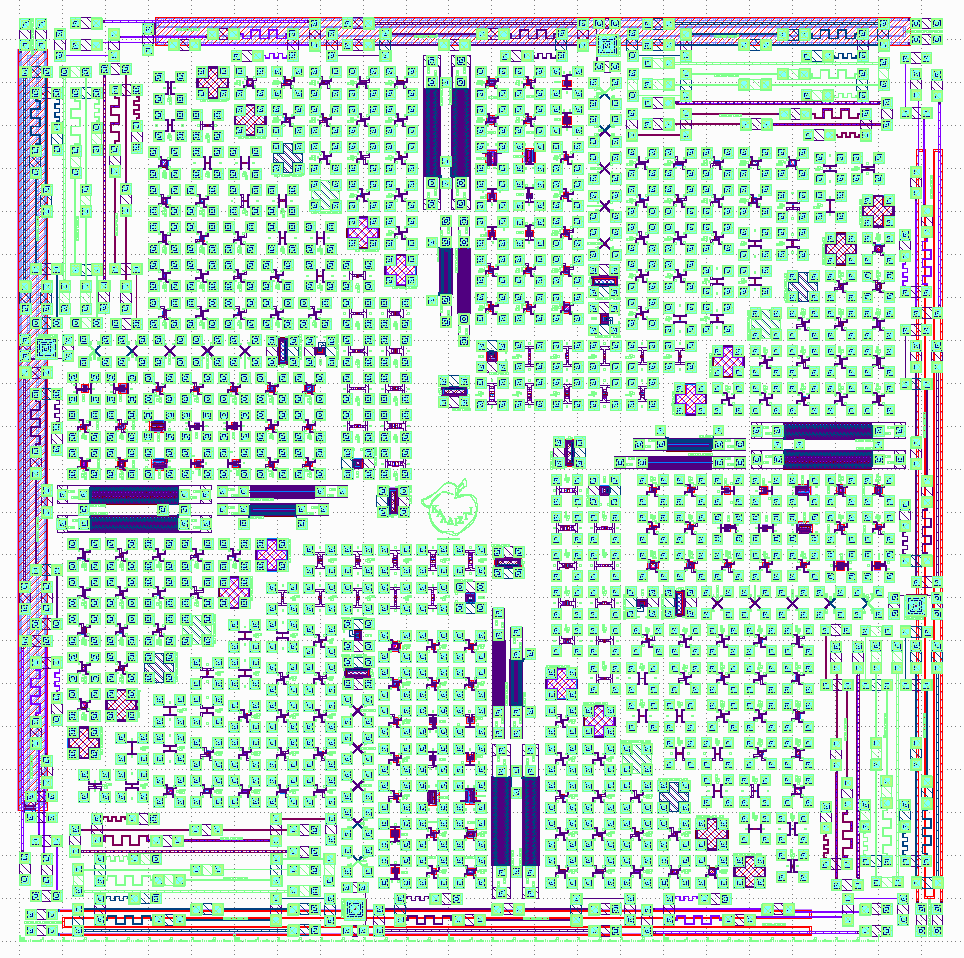
\includegraphics[width=0.4\textwidth]{images/pearlriver.png}
		\hspace{1cm}
		
\includegraphics[width=0.4\textwidth]{images/27c91467-0084-4503-9805-3b53d4d3043e.jpeg}
	\end{center}
\end{frame}

\begin{frame}{The LibreSilicon project}
	\begin{itemize}
%        \setlength\itemsep{1em}
		\item In 2017 leviathan already has found a clean room to rent at Hong Kong University of Science and Technology
		\item Last year at 34c3 he gave a Lightning Talk about LibreSilicon
		\item Since then we're meeting every week on Sunday 2100 HKT at Mumble
		\item Communicating, planing and working via mailing list and Mumble
		\item Held a tool chain hackathon end of May 2018
		\item Already two of us got qualification for clean room access at HKUST
		\item Processing our first test wafer for characterization ($\rightarrow$ pics follow)
	\end{itemize}
\end{frame}

\begin{frame}{Basic points}
	\begin{itemize}
        \setlength\itemsep{1em}
		\item Starting with 1$\mu m$ "feature size" because still well documented in text books
		\item Robust, at least 5 Volt tolerant, well suited for maker, tinkerer and hacker
		\item Twin-Well process for CMOS with 3 metal layer w/ very interesting additions
		\item Quite suitable for "low tec" in the basement
		\item For analog circuits, regarding their huge transistor sizes, small feature sizes do not matter
	\end{itemize}
\end{frame}

\begin{frame}{Main (re-)construction areas}
	\begin{enumerate}
		\item Figure out / develop the process itself ($\rightarrow$ almost done)
		\item Rebuild / modernize the tools / design flow ($\rightarrow$ ongoing)
		\item Compile / design a almost complete standard cell library ($\rightarrow$ ongoing)
	\end{enumerate}
\end{frame}

\section[Standard cells]{}
\begin{frame}{Standard Cells}
Standard Cells are usualy
	\begin{itemize}
        \setlength\itemsep{1em}
		\item A collection of some dozens of combinatorial + sequential cells
		\item Instantiated many, many times in a netlist
		\item Used also as layout primitives
	\end{itemize}
\end{frame}

\begin{frame}{Typical cells}
	\begin{figure}[h]
		\begin{center}
			\begin{circuitdiagram}{25}{25}
				\gate[\inputs{4}]{and}{-20}{20}{R}{AND4}{}
				\gate[\inputs{3}]{nand}{-10}{20}{R}{NAND3}{}
				\gate[\inputs{2}]{nand}{0}{20}{R}{NAND2}{}
				\gate[\inputs{2}]{xnor}{10}{20}{R}{EQ2}{}
				\gate[\inputs{4}]{or}{20}{20}{R}{OR4}{}
				\gate[\inputs{3}]{nor}{30}{20}{R}{NOR3}{}
				\gate[\inputs{2}]{nor}{-20}{10}{R}{NOR2}{}
				\gate[\inputs{2}]{xor}{-10}{10}{R}{XOR2}{}
				\gate{not}{0}{10}{R}{INV}{}
				\flipflop{nsr}{10}{10}{R}{SRL}{}
				\flipflop{d}{20}{10}{R}{DFF}{}
				\flipflop{njk}{30}{10}{R}{JKFF}{}
			\end{circuitdiagram}
		\end{center}
	\end{figure}

... and much more
\end{frame}

\begin{frame}{Design goals}
here are
	\begin{itemize}
        \setlength\itemsep{1em}
		\item Being almost complete (more cells $\rightarrow$ better netlist)
		\item Being low energy consuming (less Watts per square)
		\item Being as fast as possible (w/ small timing delay)
		\item Having a small footprint (small cell size)
	\end{itemize}

Well, does not fit all together well.
\end{frame}

\begin{frame}{Cell representations}
every single cell needs different representation for working smooth with different tools, e.g.
	\begin{itemize}
		\item For simulation ($\rightarrow$ Verilog and Spice)
		\item For synthesis ($\rightarrow$ Liberty file format)
		\item For timing ($\rightarrow$ standard delay format)
		\item For layout ($\rightarrow$ library exchange format)
		\item Or, even for dedicated tools (e.g. Magic)
		\item And documentation (schematics, truth tables, data sheets, ..)
	\end{itemize}
\end{frame}

\begin{frame}{Cell representations}
Regarding our goal of several hundreds cells (estimated 300+), generating \textbf{all} cell representations, becomes a huge task.

Nobody likes to do this manually.

We need a tool for that!

A cell generator.

\end{frame}

\begin{frame}{Cell generator}
This cell generator, named "Popcorn", is still work-in-progress.

Starting from one source this tool

	\begin{itemize}
		\item Should generate all representation formats
		\item Already helps drawing the schematics
		\item Already generates a couple of data sheet like LaTeX file
		\item Was written in Tcl first, but
		\item Needs a rewrite in a more sophisticated / AI-ish language
		\item Now when test wafer characterization is done
	\end{itemize}
\end{frame}

\begin{frame}{Standard cell library}
	\begin{itemize}
        \setlength\itemsep{1em}
		\item https://www.github.com/chipforge/StdCellLib ($\rightarrow$ repository)
		\item https://vcs.in-berlin.de/chipforge\_stdcelllib/index ($\rightarrow$ wiki)
	\end{itemize}

maintained by chipforge
\end{frame}

\section[Silicon compiler]{}
\begin{frame}{Open source tools}
	\begin{itemize}
        \setlength\itemsep{1em}
		\item yosys
		\item graywolf
		\item qrouter
		\item several FPGA routers
	\end{itemize}
\end{frame}

\begin{frame}{graywolf}
	\begin{itemize}
        \setlength\itemsep{1em}
		\item Originates in academia: TimberWolf
		\item Simulated annealing
	        \begin{itemize}
		    \item Meta heuristic that is useful not only for placement
	        \end{itemize}
		\item Inline syscalls
	        \begin{itemize}
		    \item This is just a bad idea
	        \end{itemize}
	\end{itemize}
\end{frame}

\begin{frame}{qrouter}
	\begin{itemize}
        \setlength\itemsep{1em}
		\item Started in 2011 by Tim Edwards 
		\item Widely used for FPGA
	        \begin{itemize}
		    \item Not ready for silicon
	        \end{itemize}
		\item Sequential routing
	        \begin{itemize}
		    \item Parallelism not in scope
	        \end{itemize}
		\item Difficult to prove formal correctness
	        \begin{itemize}
		    \item Prove that C implementation of rip-up and re-route is correct
	        \end{itemize}
	\end{itemize}
\end{frame}

\begin{frame}{Productive tools}
	\begin{itemize}
        \setlength\itemsep{1em}
		\item Different tool sets like BonnRoute, Cadence suite, Alliance tools, etc.
		\item Similar capabilities with respect to silicon
		\item Just throw man-power at VLSI --- what is automation?
	\end{itemize}
\end{frame}

{
\setbeamercolor{background canvas}{bg=black}
\begin{frame}
    \begin{center}
        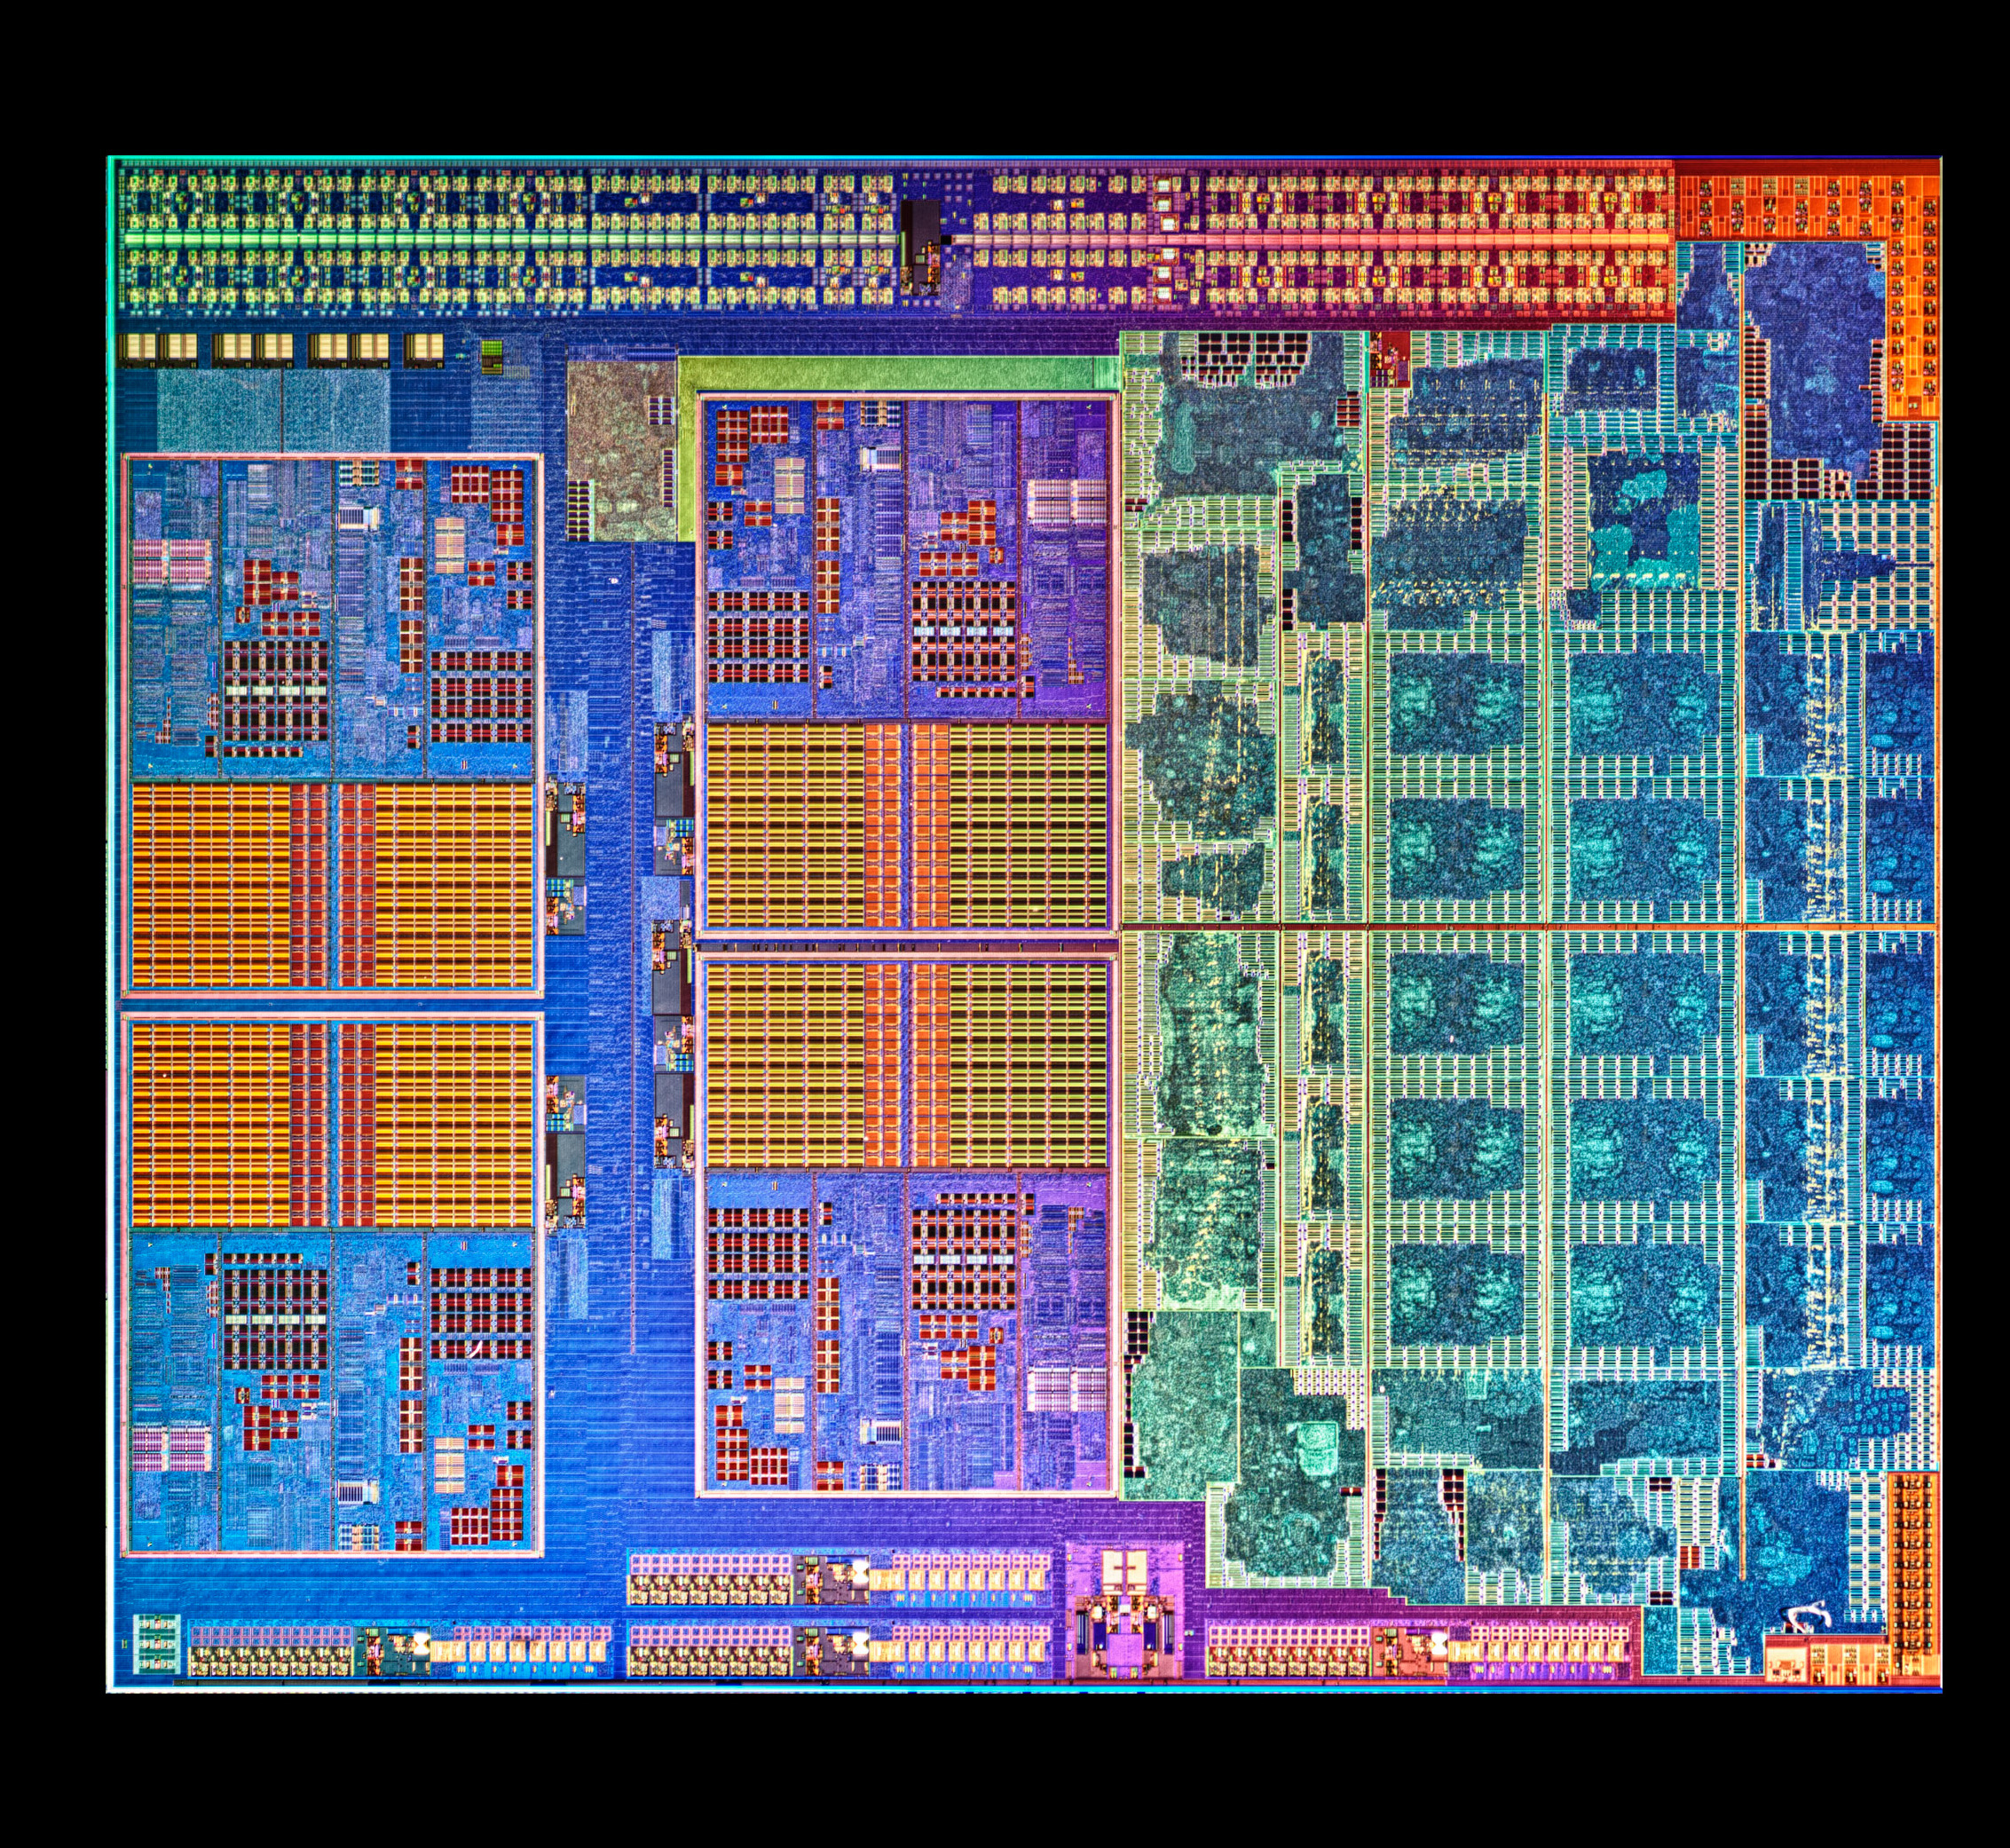
\includegraphics[height=\textheight]{images/VLSI01_rotated.jpg}
    \end{center}
\end{frame} 
}

\begin{frame}{Routing: State of the art}
	\begin{itemize}
        \setlength\itemsep{1em}
		\item Place components for a large chip
		\item Route wires roughly along a chessboard for a large chip
		\item Route detailed tracks and vias for a large chip
		\item Formal correctness: Rip-up and Re-route
		\item Formal style: Sequential/Imperative code
	\end{itemize}
\end{frame}

\begin{frame}{Routing: Proposed}
	\begin{itemize}
        \setlength\itemsep{1em}
		\item Decomposition for a large chip
		\item Place components and route for small chips in parallel
		\item Place abstract gates and route recursively
		\item Formal correctness: Reduction from SMT
		\item Formal style: Parallel/Declarative code
	\end{itemize}
\end{frame}

\begin{frame}{Divide and Conquer}
	    \textbf{Academia + Industry:}
	    \begin{itemize}
		\item Placement and Routing are different problems
		\item All components map to the same problem
	    \end{itemize}
	    \textbf{LibreSilicon:}
	    \begin{itemize}
		\item Placement and Routing are the same problem
		\item Different components map to different problems
	    \end{itemize}
\end{frame}

\begin{frame}{Routing Hierarchy}
	    \textbf{Academia + Industry:}
	    \begin{itemize}
		\item Geographical partitioning of a wafer $\rightarrow$ \textit{cut tree}
		\item Based on preceeding placement steps
	    \end{itemize}
	    \textbf{LibreSilicon:}
	    \begin{itemize}
		\item Modular chip development $\rightarrow$ \textit{subcell hierarchy}
		\item Subcells carry implicit and explicit subcells
	    \end{itemize}
\end{frame}

\begin{frame}{Frontier: Parallelism}
	\begin{itemize}
        \setlength\itemsep{1em}
		\item BonnRoute: concurrency + shared memory model
		\item qrouter: none 
		\item lsc: map + reduce
	\end{itemize}
\end{frame}

\begin{frame}{Subcell hierarchies}
	\begin{itemize}
        \setlength\itemsep{1em}
		\item Explicit subcell hierarchies through high modularization
		\item Implicit subcell hierarchies through exlining
		\item Preserve hierarchy in compiler interfaces
	\end{itemize}
\end{frame}

\begin{frame}{High modularization}
        \begin{figure}
        \centering
        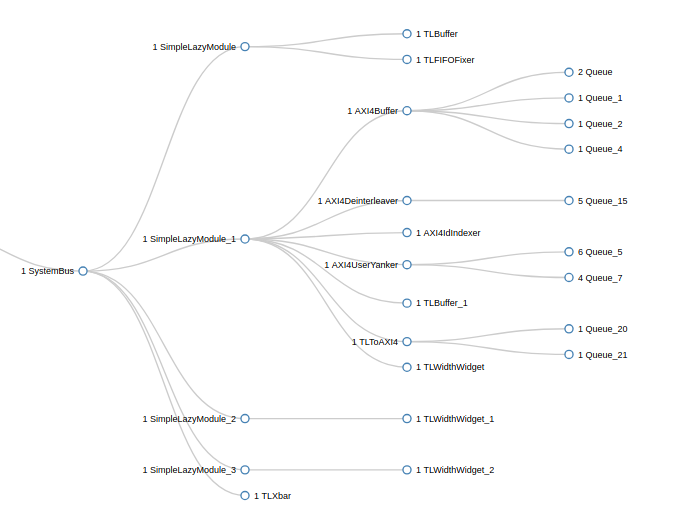
\includegraphics[scale=0.42]{images/SystemBus.png}
        \end{figure}
        \begin{center}
            \href{url}{\scalebox{0.5}{https://murmur.libresilicon.com/lsc/rocket-chip-yosys}}
        \end{center}
\end{frame}

\begin{frame}{Exlining}
	\begin{itemize}
        \setlength\itemsep{1em}
		\item Proof of concept: picorv
	\end{itemize}
        \begin{center}
            \href{url}{\scalebox{0.5}{https://murmur.libresilicon.com/lsc/rocket-chip-exline}}
        \end{center}
\end{frame}

\begin{frame}{Unconstrained Small Unified Silicon Problem}
	\begin{itemize}
        \setlength\itemsep{1em}
		\item Components and nets $\rightarrow$ \textit{rectilinear geometries}
		\item Components do not overlap
		\item Nets overlap with their pins on components
	\end{itemize}
\end{frame}

\begin{frame}{Minimizing Goals}
	\begin{itemize}
        \setlength\itemsep{1em}
		\item Layout area
		\item Maximum wire length 
		\item Via count
		\item Crossing number (computational)
		\item Wire jogs (minor)
	\end{itemize}
\end{frame}

\begin{frame}{Satisfiability Modulo Theories}
	\begin{itemize}
        \setlength\itemsep{1em}
            \item Optimization problems
            \item Abstraction from Boolean satisfiability
            \item Several solvers implement smtlib2
	    \begin{itemize}
                \item \textit{ABC} from University of Berkeley
                \item \textit{CVC4} from Stanford
                \item \textit{Boolector} from Johannes Kepler University
                \item \textit{MathSAT} from Fondazione Bruno Kessler and DISI-University of Trento
                \item \textit{Yices} from SRI
                \item \textit{Z3} from Microsoft
	    \end{itemize}
	\end{itemize}
\end{frame}

\begin{frame}{Boolean Satisfiability}
    \begin{center}
        $ ( \alpha_{1} \vee \alpha_{2} \vee \alpha_{3} )
    \land ( \neg \alpha_{4} \vee \alpha_{5} \vee \alpha_{6} )
        $
    \end{center}
\end{frame}

\begin{frame}{Defining rectangular components}
	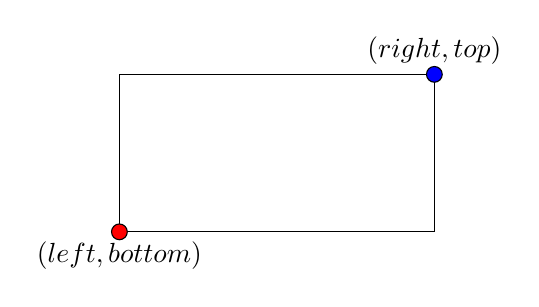
\begin{tikzpicture}
            \draw (0,-8) rectangle (4,-6);
            \draw[fill=red]  (0,-8) circle (0.1);
            \draw[fill=blue] (4,-6) circle (0.1);
            \node at (0,-8.3) {$(left, bottom)$};
            \node at (4,-5.7) {$(right, top)$};
	\end{tikzpicture}
\end{frame}

\begin{frame}{Overlaps}
	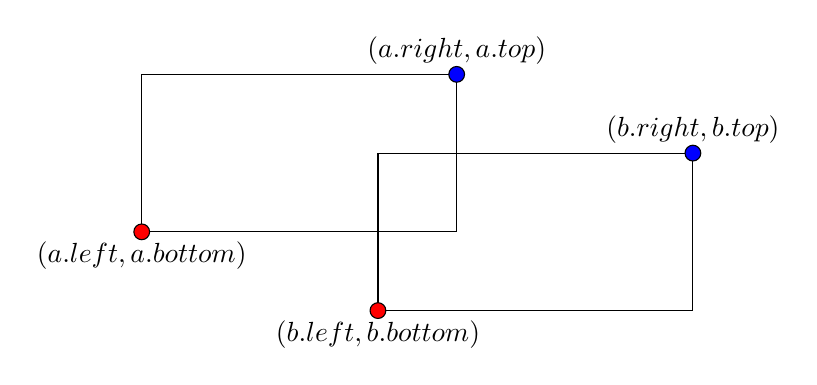
\begin{tikzpicture}
            \draw (0,-8) rectangle (4,-6);
            \draw[fill=red]  (0,-8) circle (0.1);
            \draw[fill=blue] (4,-6) circle (0.1);
            \node at (0,-8.3) {$(a.left, a.bottom)$};
            \node at (4,-5.7) {$(a.right, a.top)$};
            
            \draw (3,-9) rectangle (7,-7);
            \draw[fill=red]  (3,-9) circle (0.1);
            \draw[fill=blue] (7,-7) circle (0.1);
            \node at (3,-9.3) {$(b.left, b.bottom)$};
            \node at (7,-6.7) {$(b.right, b.top)$};
	\end{tikzpicture}
\end{frame}

\begin{frame}{Reduction from SMT}
    \begin{center}
        $ a.right - a.left = dimension.x  $ \\
        $ b.right - b.left = dimension.y  $ \\

        $ a.top - a.bottom = dimension.x $ \\
        $ b.top - b.bottom = dimension.y $ \\~\\

        $ \phantom{\lor}\phantom{tm} b.left > a.right $ \\
        $ \lor\phantom{tm} a.left > b.right $ \\
        $ \lor a.bottom > b.top $ \\
        $ \lor b.bottom > a.top $ \\
    \end{center}
\end{frame}

\begin{frame}{Combining in the LSC Semigroup}
    \begin{center}
        overlaps + pin connect + arbitrary constraint
    \end{center}
\end{frame}

\begin{frame}{Stay low}
    \begin{tikzpicture}
        \begin{axis}
          [ xticklabels={,,}
          , yticklabels={,,}
          , scaled ticks=false
          , xmin=0,ymin=0
          , samples=123
          , domain=0:42
          , width=1.1\textwidth,
          , height=0.55\textwidth
          ]
        \addplot[blue] {pow(2,x)} node[above]{};
        \end{axis}
    \end{tikzpicture}
\end{frame}

\begin{frame}{Maximize yield}
	\begin{itemize}
        \setlength\itemsep{1em}
		\item Minimize area of a chip $\rightarrow$ \textit{silicon compiler}
		\item Minimize physical errors $\rightarrow$ \textbf{silicon process}
	\end{itemize}
\end{frame}

\begin{frame}{Libre Silicon Compiler}
	\begin{itemize}
        \setlength\itemsep{1em}
		\item https://www.github.com/foshardware/lsc ($\rightarrow$ repository)
	\end{itemize}

maintained by foshardware
\end{frame}

\section[Process]{}

\begin{frame}{Why Hong Kong?}
	\begin{center}
		 \textbf{History}

		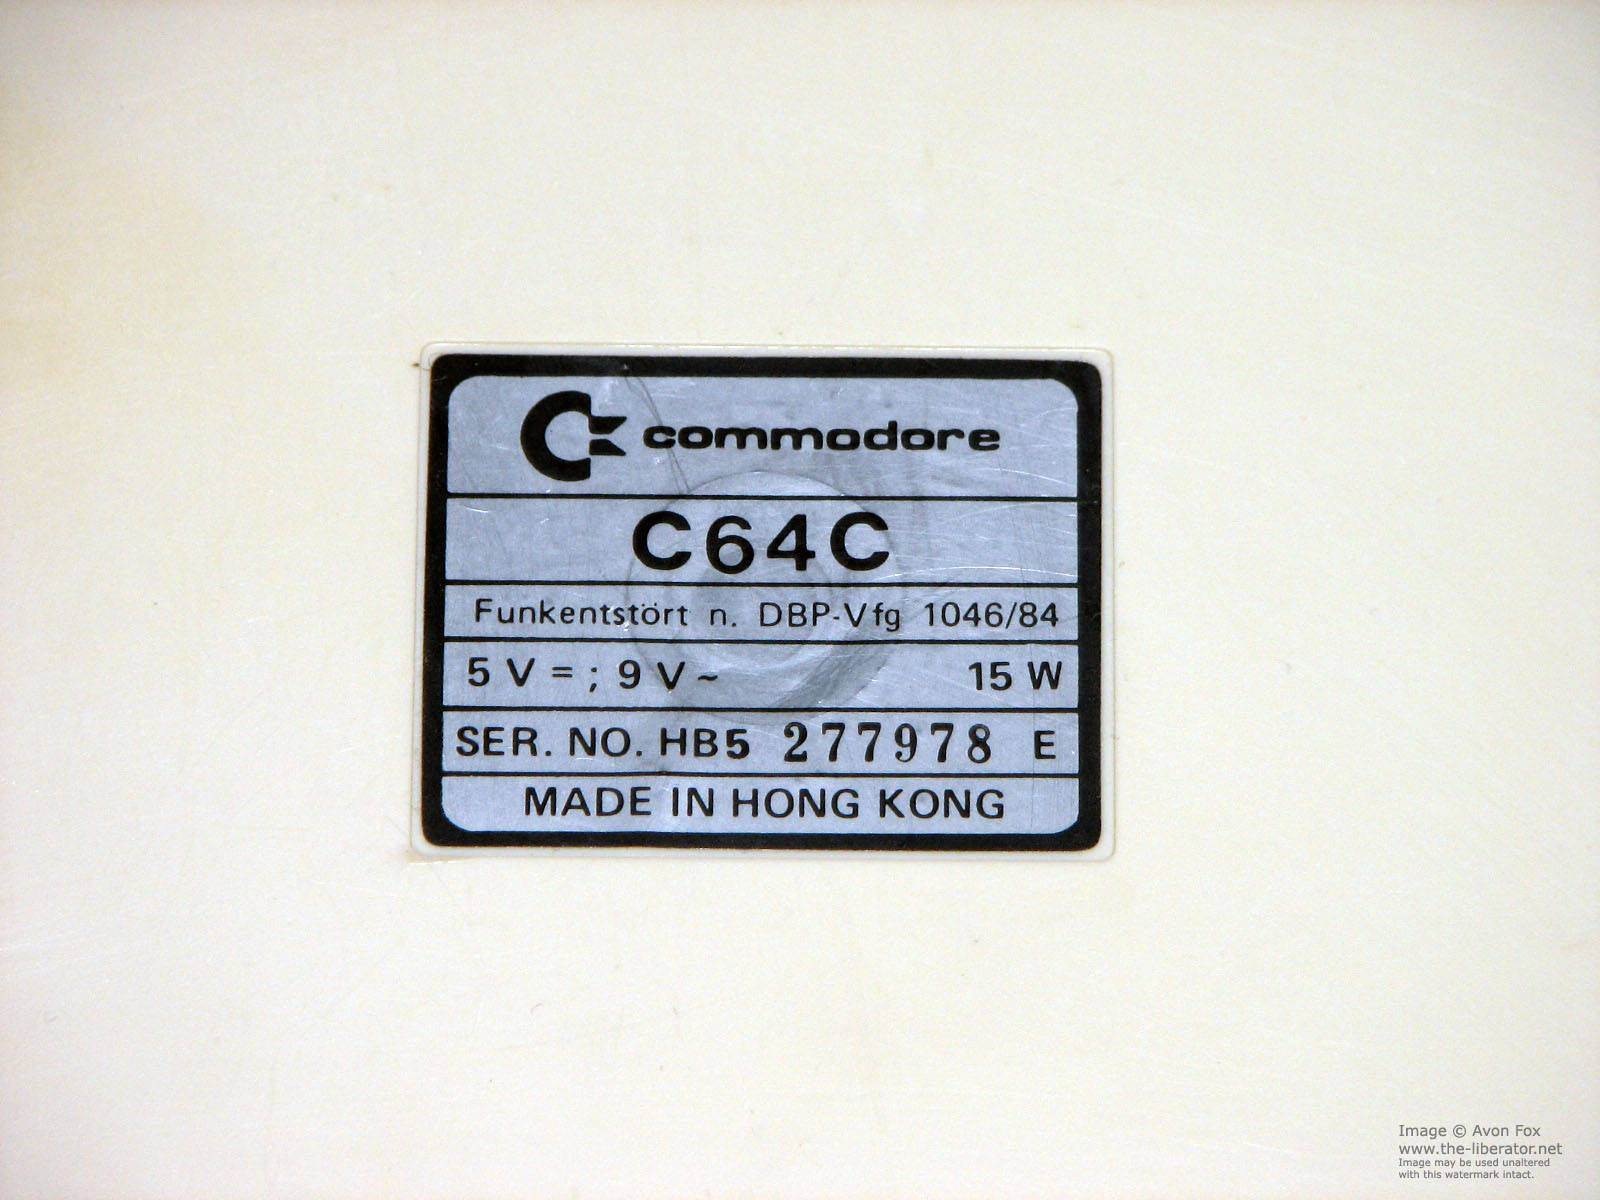
\includegraphics[height=0.7\textheight]{images/15443222_1411927645507464_7594635994572097245_o.jpg}
	\end{center}
\end{frame}

\begin{frame}{Why Hong Kong?}
	\begin{center}
		
\includegraphics[width=0.4\textwidth]{images/u=3232688716,3661225619&fm=26&gp=0.jpg}
		
		\textbf{Nano fabrication facility}
	\end{center}
\end{frame}

\begin{frame}{Why Hong Kong?}
	\begin{center}
		
\includegraphics[width=0.4\textwidth]{images/RCL.jpg}
		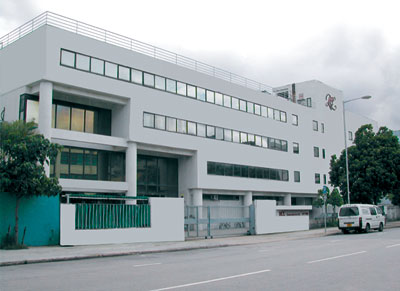
\includegraphics[width=0.4\textwidth]{images/factory.jpg}
	\end{center}
\end{frame}

\begin{frame}{Why Hong Kong?}
	\textbf{Conclusion}
	\begin{itemize}
		\item Advanced labs available for R\&D
		\item Shenzhen and Hong Kong have fabs which are willing to introduce LibreSilicon
		\item Channels for easy export to Europe already established (One belt, one road)
		\item Climate is better
		\item Payment is better
		\item Food is better
		\item * is better
		\item The sun shines brightest in the east ;-)
	\end{itemize}
\end{frame}

\begin{frame}{Features}
	\begin{itemize}
        \setlength\itemsep{1em}
		\item MOSFETs
		\item LDMOSFETs (High voltage) 
		\item BJTs
		\item Zener polysilicon diodes
		\item SONOS flash cells
		\item Polysilicon resistors
		\item Metal caps
	\end{itemize}
\end{frame}

\begin{frame}{Process design considerations}
	\begin{itemize}
		\item Should be portable
		\item Robust
		\item Low amount of layers
		\item KISS (Keep it simple and stupid)
		\item Avoid expensive machines
		\item Can be manufactured in a home lab
	\end{itemize}
\end{frame}

\begin{frame}{Process design considerations}
	\begin{center}
		
\includegraphics[height=0.8\textheight]{images/breaking-bad.png}
	\end{center}
\end{frame}

\begin{frame}{Process design considerations}
	\begin{center}
		
\includegraphics[height=0.8\textheight]{images/innovation-hub-hamburg.jpg}
	\end{center}
\end{frame}

\begin{frame}{Cross section}
	\begin{center}
		\begin{tikzpicture}[node distance = 3cm, auto, thick,scale=0.25, every node/.style={transform shape}]
			\fill[isolationoxide] (0.0,\LowerMoreMetalTwo) rectangle (55.0,\UpperGlass);

\fill[isolationoxide] (0.0,\LowerMoreMetal) rectangle (55.0,\LowerMoreMetalTwo);

\input{tikz_process_steps/more_metal.a.tex}

\fill[white] (2.75,\UpperMoreMetal) rectangle (4.25,\LowerMoreMetalTwo);
\fill[white] (5.50,\UpperMoreMetal) rectangle (7.0,\LowerMoreMetalTwo);
\fill[white] (8.25,\UpperMoreMetal) rectangle (9.75,\LowerMoreMetalTwo);
\fill[white] (11.00,\UpperMoreMetal) rectangle (12.5,\LowerMoreMetalTwo);
\fill[white] (13.75,\UpperMoreMetal) rectangle (15.25,\LowerMoreMetalTwo);

\fill[white] (20.35,\UpperMoreMetal) rectangle (21.65,\LowerMoreMetalTwo);
\fill[white] (22.60,\UpperMoreMetal) rectangle (23.90,\LowerMoreMetalTwo);
\fill[white] (24.35,\UpperMoreMetal) rectangle (25.65,\LowerMoreMetalTwo);

\fill[white] (26.35,\UpperMoreMetal) rectangle (27.65,\LowerMoreMetalTwo);
\fill[white] (28.10,\UpperMoreMetal) rectangle (29.15,\LowerMoreMetalTwo);
\fill[white] (29.60,\UpperMoreMetal) rectangle (30.65,\LowerMoreMetalTwo);
\fill[white] (31.10,\UpperMoreMetal) rectangle (32.15,\LowerMoreMetalTwo);
\fill[white] (32.60,\UpperMoreMetal) rectangle (33.90,\LowerMoreMetalTwo);

\fill[white] (35.10,\UpperMoreMetal) rectangle (36.15,\LowerMoreMetalTwo);
\fill[white] (36.85,\UpperMoreMetal) rectangle (37.90,\LowerMoreMetalTwo);
\fill[white] (38.35,\UpperMoreMetal) rectangle (39.40,\LowerMoreMetalTwo);
\fill[white] (39.85,\UpperMoreMetal) rectangle (40.90,\LowerMoreMetalTwo);
\fill[white] (41.15,\UpperMoreMetal) rectangle (42.15,\LowerMoreMetalTwo);

\fill[white] (43.0,\UpperMoreMetal) rectangle (44.5,\LowerMoreMetalTwo);
\fill[white] (46.5,\UpperMoreMetal) rectangle (48.0,\LowerMoreMetalTwo);

\fill[white] (48.75,\UpperMoreMetal) rectangle (50.25,\LowerMoreMetalTwo);
\fill[white] (52.75,\UpperMoreMetal) rectangle (54.25,\LowerMoreMetalTwo);


\fill[metal3] (2.75,\UpperMoreMetal) rectangle (4.25,\LowerMoreMetalTwo);
\fill[metal3] (5.50,\UpperMoreMetal) rectangle (7.0,\LowerMoreMetalTwo);
\fill[metal3] (8.25,\UpperMoreMetal) rectangle (9.75,\LowerMoreMetalTwo);
\fill[metal3] (11.00,\UpperMoreMetal) rectangle (12.5,\LowerMoreMetalTwo);
\fill[metal3] (13.75,\UpperMoreMetal) rectangle (15.25,\LowerMoreMetalTwo);

\fill[metal3] (20.35,\UpperMoreMetal) rectangle (21.65,\LowerMoreMetalTwo);
\fill[metal3] (22.60,\UpperMoreMetal) rectangle (23.90,\LowerMoreMetalTwo);
\fill[metal3] (24.35,\UpperMoreMetal) rectangle (25.65,\LowerMoreMetalTwo);

\fill[metal3] (26.35,\UpperMoreMetal) rectangle (27.65,\LowerMoreMetalTwo);
\fill[metal3] (28.10,\UpperMoreMetal) rectangle (29.15,\LowerMoreMetalTwo);
\fill[metal3] (29.60,\UpperMoreMetal) rectangle (30.65,\LowerMoreMetalTwo);
\fill[metal3] (31.10,\UpperMoreMetal) rectangle (32.15,\LowerMoreMetalTwo);
\fill[metal3] (32.60,\UpperMoreMetal) rectangle (33.90,\LowerMoreMetalTwo);

\fill[metal3] (35.10,\UpperMoreMetal) rectangle (36.15,\LowerMoreMetalTwo);
\fill[metal3] (36.85,\UpperMoreMetal) rectangle (37.90,\LowerMoreMetalTwo);
\fill[metal3] (38.35,\UpperMoreMetal) rectangle (39.40,\LowerMoreMetalTwo);
\fill[metal3] (39.85,\UpperMoreMetal) rectangle (40.90,\LowerMoreMetalTwo);
\fill[metal3] (41.15,\UpperMoreMetal) rectangle (42.15,\LowerMoreMetalTwo);

\fill[metal3] (43.0,\UpperMoreMetal) rectangle (44.5,\LowerMoreMetalTwo);
\fill[metal3] (46.5,\UpperMoreMetal) rectangle (48.0,\LowerMoreMetalTwo);

\fill[metal3] (48.75,\UpperMoreMetal) rectangle (50.25,\LowerMoreMetalTwo);
\fill[metal3] (52.75,\UpperMoreMetal) rectangle (54.25,\LowerMoreMetalTwo);

% wire
\fill[metal3] ( 2.50,\LowerMoreMetalTwo) rectangle ( 4.50,\UpperMoreMetalTwo);
\fill[metal3] ( 5.25,\LowerMoreMetalTwo) rectangle ( 7.25,\UpperMoreMetalTwo);
\fill[metal3] ( 8.00,\LowerMoreMetalTwo) rectangle (10.00,\UpperMoreMetalTwo);
\fill[metal3] (10.75,\LowerMoreMetalTwo) rectangle (12.75,\UpperMoreMetalTwo);
\fill[metal3] (13.50,\LowerMoreMetalTwo) rectangle (15.50,\UpperMoreMetalTwo);

\fill[metal3] (20.00,\LowerMoreMetalTwo) rectangle (22.00,\UpperMoreMetalTwo);
\fill[metal3] (22.50,\LowerMoreMetalTwo) rectangle (24.00,\UpperMoreMetalTwo);
\fill[metal3] (24.25,\LowerMoreMetalTwo) rectangle (25.75,\UpperMoreMetalTwo);

\fill[metal3] (26.15,\LowerMoreMetalTwo) rectangle (27.75,\UpperMoreMetalTwo);
\fill[metal3] (28.00,\LowerMoreMetalTwo) rectangle (29.25,\UpperMoreMetalTwo);
\fill[metal3] (29.50,\LowerMoreMetalTwo) rectangle (30.75,\UpperMoreMetalTwo);
\fill[metal3] (30.95,\LowerMoreMetalTwo) rectangle (32.30,\UpperMoreMetalTwo);
\fill[metal3] (32.50,\LowerMoreMetalTwo) rectangle (34.25,\UpperMoreMetalTwo);

\fill[metal3] (34.75,\LowerMoreMetalTwo) rectangle (36.25,\UpperMoreMetalTwo);
\fill[metal3] (36.50,\LowerMoreMetalTwo) rectangle (38.00,\UpperMoreMetalTwo);
\fill[metal3] (38.25,\LowerMoreMetalTwo) rectangle (39.50,\UpperMoreMetalTwo);
\fill[metal3] (39.75,\LowerMoreMetalTwo) rectangle (40.95,\UpperMoreMetalTwo);
\fill[metal3] (41.10,\LowerMoreMetalTwo) rectangle (42.35,\UpperMoreMetalTwo);

\fill[metal3] (42.75,\LowerMoreMetalTwo) rectangle (44.75,\UpperMoreMetalTwo);
\fill[metal3] (46.25,\LowerMoreMetalTwo) rectangle (48.25,\UpperMoreMetalTwo);

\fill[metal3] (48.50,\LowerMoreMetalTwo) rectangle (50.50,\UpperMoreMetalTwo);
\fill[metal3] (52.50,\LowerMoreMetalTwo) rectangle (54.50,\UpperMoreMetalTwo);



\fill[white] ( 2.65,\UpperMoreMetalTwo) rectangle ( 4.35,\UpperGlass);
\fill[white] ( 5.35,\UpperMoreMetalTwo) rectangle ( 7.15,\UpperGlass);
\fill[white] ( 8.10,\UpperMoreMetalTwo) rectangle ( 9.90,\UpperGlass);
\fill[white] (10.85,\UpperMoreMetalTwo) rectangle (12.65,\UpperGlass);
\fill[white] (13.60,\UpperMoreMetalTwo) rectangle (15.40,\UpperGlass);

\fill[white] (20.10,\UpperMoreMetalTwo) rectangle (21.90,\UpperGlass);
\fill[white] (22.60,\UpperMoreMetalTwo) rectangle (23.90,\UpperGlass);
\fill[white] (24.35,\UpperMoreMetalTwo) rectangle (25.65,\UpperGlass);

\fill[white] (26.25,\UpperMoreMetalTwo) rectangle (27.65,\UpperGlass);
\fill[white] (28.10,\UpperMoreMetalTwo) rectangle (29.15,\UpperGlass);
\fill[white] (29.60,\UpperMoreMetalTwo) rectangle (30.65,\UpperGlass);
\fill[white] (31.10,\UpperMoreMetalTwo) rectangle (32.20,\UpperGlass);
\fill[white] (32.60,\UpperMoreMetalTwo) rectangle (34.15,\UpperGlass);

\fill[white] (34.85,\UpperMoreMetalTwo) rectangle (36.15,\UpperGlass);
\fill[white] (36.60,\UpperMoreMetalTwo) rectangle (37.90,\UpperGlass);
\fill[white] (38.35,\UpperMoreMetalTwo) rectangle (39.40,\UpperGlass);
\fill[white] (39.85,\UpperMoreMetalTwo) rectangle (40.85,\UpperGlass);
\fill[white] (41.20,\UpperMoreMetalTwo) rectangle (42.25,\UpperGlass);

\fill[white] (43.00,\UpperMoreMetalTwo) rectangle (44.50,\UpperGlass);
\fill[white] (46.50,\UpperMoreMetalTwo) rectangle (48.00,\UpperGlass);

\fill[white] (48.75,\UpperMoreMetalTwo) rectangle (50.25,\UpperGlass);
\fill[white] (52.75,\UpperMoreMetalTwo) rectangle (54.25,\UpperGlass);


			\node at (5,-0.5) {\textbf{\huge{PMOS}}};
			\node at (13,-0.5) {\textbf{\huge{NMOS}}};
			\node at (22,-0.5) {\textbf{\huge{SONOS flash cell (PMOS)}}};
			\node at (30,-0.5) {\textbf{\huge{NPN BJT}}};
			\node at (38,-0.5) {\textbf{\huge{PNP BJT}}};
			\node at (46,-0.5) {\textbf{\huge{Polysilicon diode}}};
			\node at (52,-0.5) {\textbf{\huge{Polyresistor}}};
		\end{tikzpicture}
	\end{center}
\end{frame}

\begin{frame}{PearlRiver \cjkfont(珠江芯片一号)}
    \begin{center}
        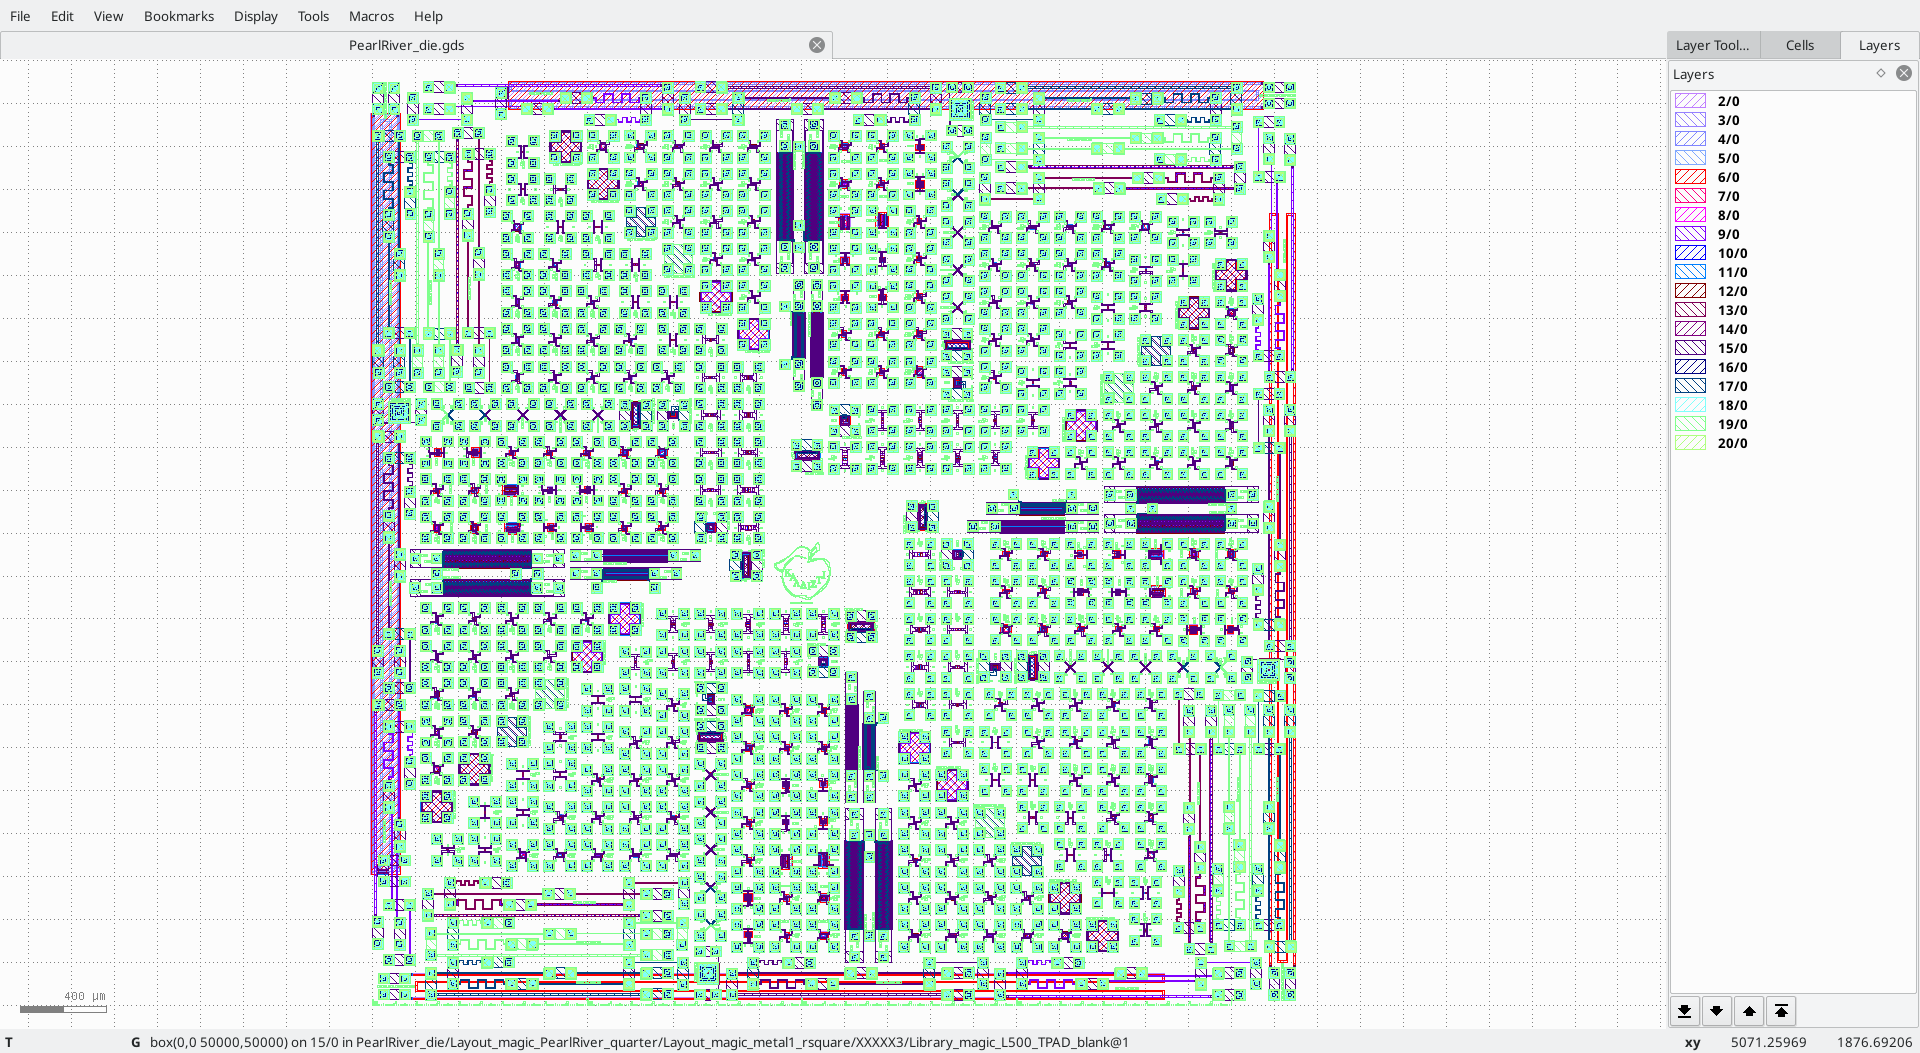
\includegraphics[height=0.8\textheight]{images/Screenshot_20181216_204924.png}
    \end{center}
\end{frame}

\begin{frame}{PearlRiver \cjkfont(珠江芯片一号)}
	\textbf{Fulfills following functions:}
	\begin{itemize}
		\item Debugging
		\item Calibration of new equipment to LibreSilicon
		\item Research of new features
		\item Syncing process features between fabs
	\end{itemize}
\end{frame}

\begin{frame}{Photomask}
	\begin{center}
		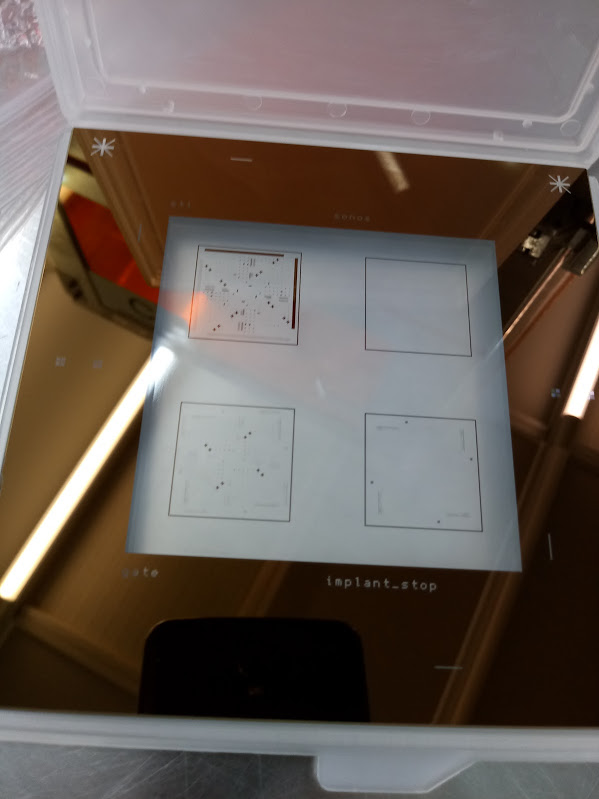
\includegraphics[height=0.8\textheight]{images/20181207_113845_Burst01.jpg}
	\end{center}
\end{frame}

\begin{frame}{Photomask}
	\begin{itemize}
		\item Is stepper/aligner brand specific
		\item ASML stepper masks contain 4 layers each
		\item The NFF stepper has a reduction value of 5:1
		\item A 5 micron gate on the mask is 1 micron on the wafer
	\end{itemize}
\end{frame}

\begin{frame}{Photo resist (HKUST)}
	\begin{center}
		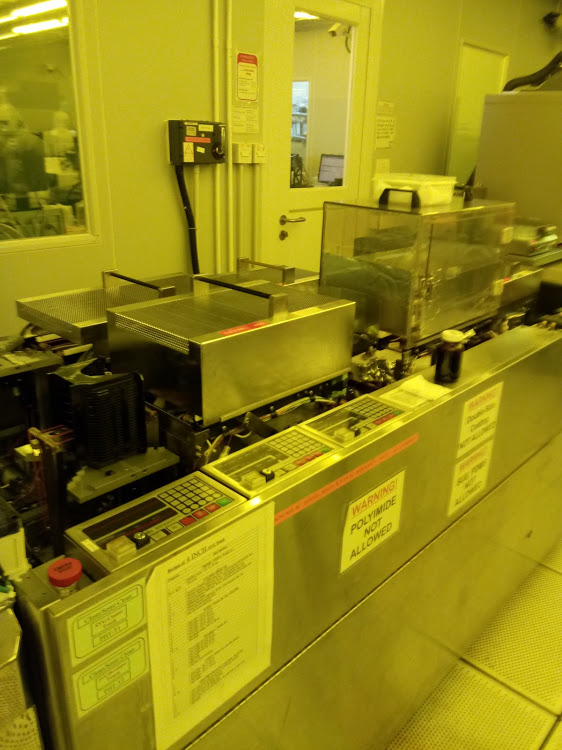
\includegraphics[height=0.8\textheight]{images/20181128_154907.jpg}
		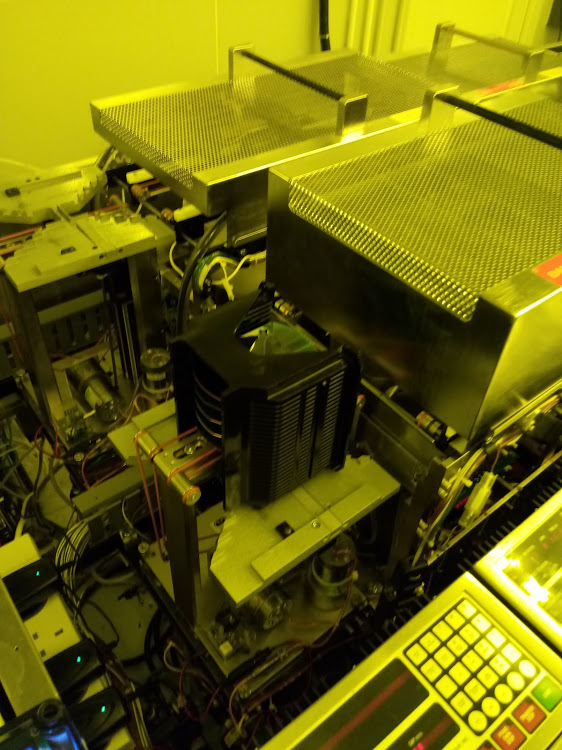
\includegraphics[height=0.8\textheight]{images/20181128_154911.jpg}
	\end{center}
\end{frame}

\begin{frame}{Photo resist (HKUST)}
	\textbf{Two types of photo resist:}
	\begin{itemize}
		\item FH 6400L (implantation)
		\item HPR 504 (normal etch)
	\end{itemize}

	\textbf{Factors to consider:}
	\begin{itemize}
		\item Thickness of FH 6400L and implantation energy are interlinked
		\item Thickness of HPR 504 and etching time are interlinked (selectivity)
	\end{itemize}
\end{frame}

\begin{frame}{After exposure}
	\begin{center}
		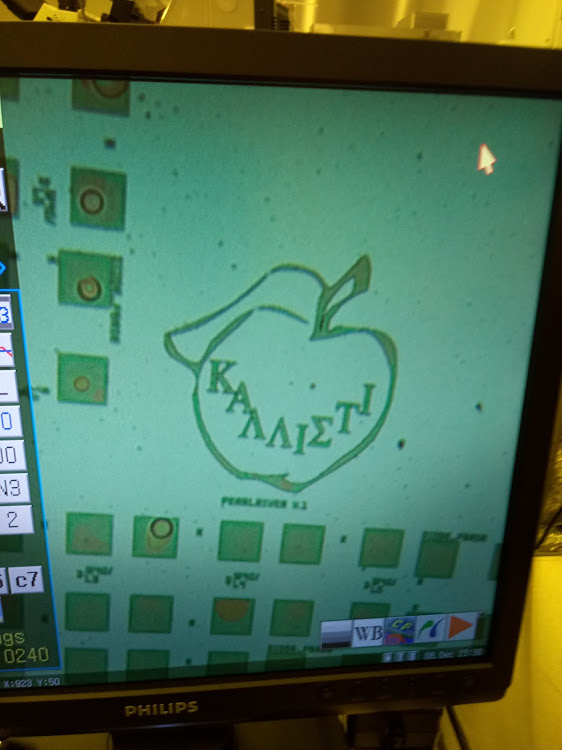
\includegraphics[height=0.8\textheight]{images/20181210_125830_Burst01.jpg}
		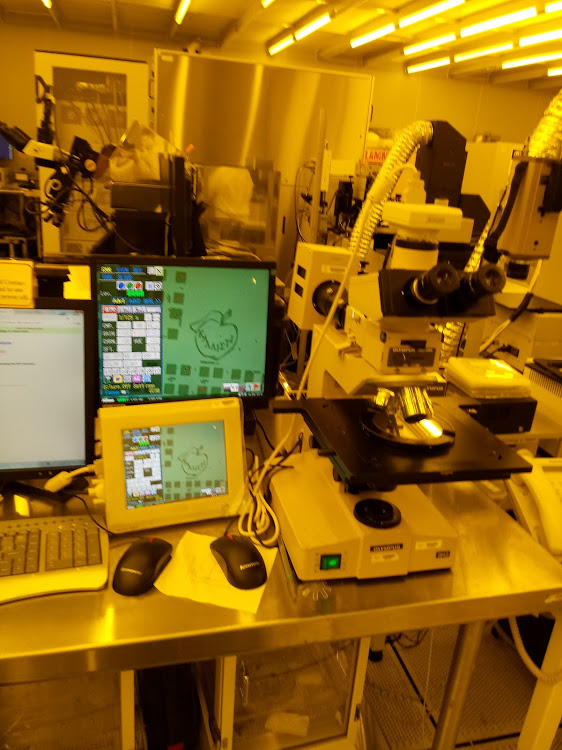
\includegraphics[height=0.8\textheight]{images/20181210_125845.jpg}
	\end{center}
\end{frame}

\begin{frame}{Alignment}
	\begin{center}
		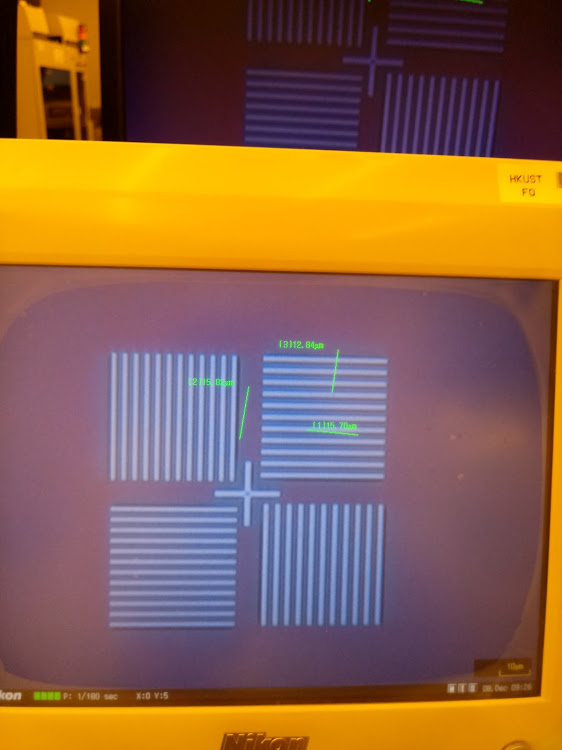
\includegraphics[height=0.8\textheight]{images/20181211_125918.jpg}
		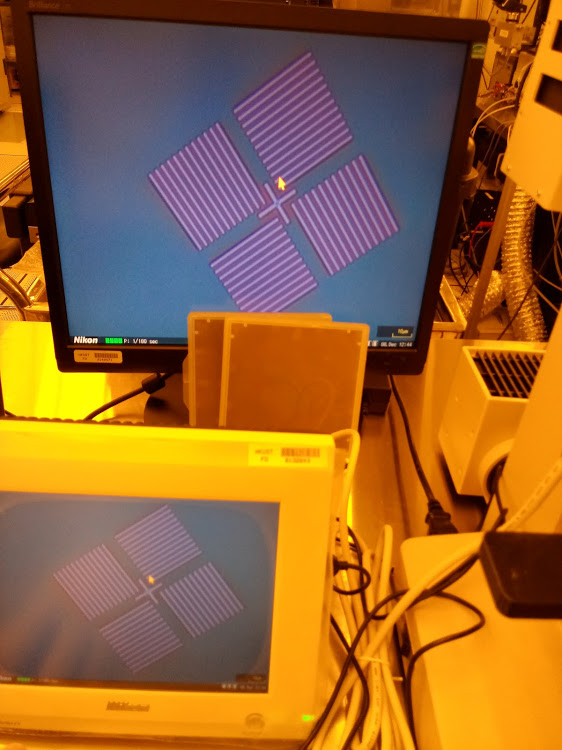
\includegraphics[height=0.8\textheight]{images/20181211_161801_Burst01.jpg}
	\end{center}
\end{frame}

\begin{frame}{Example: NOR3 ring oscillator}
	\begin{center}
		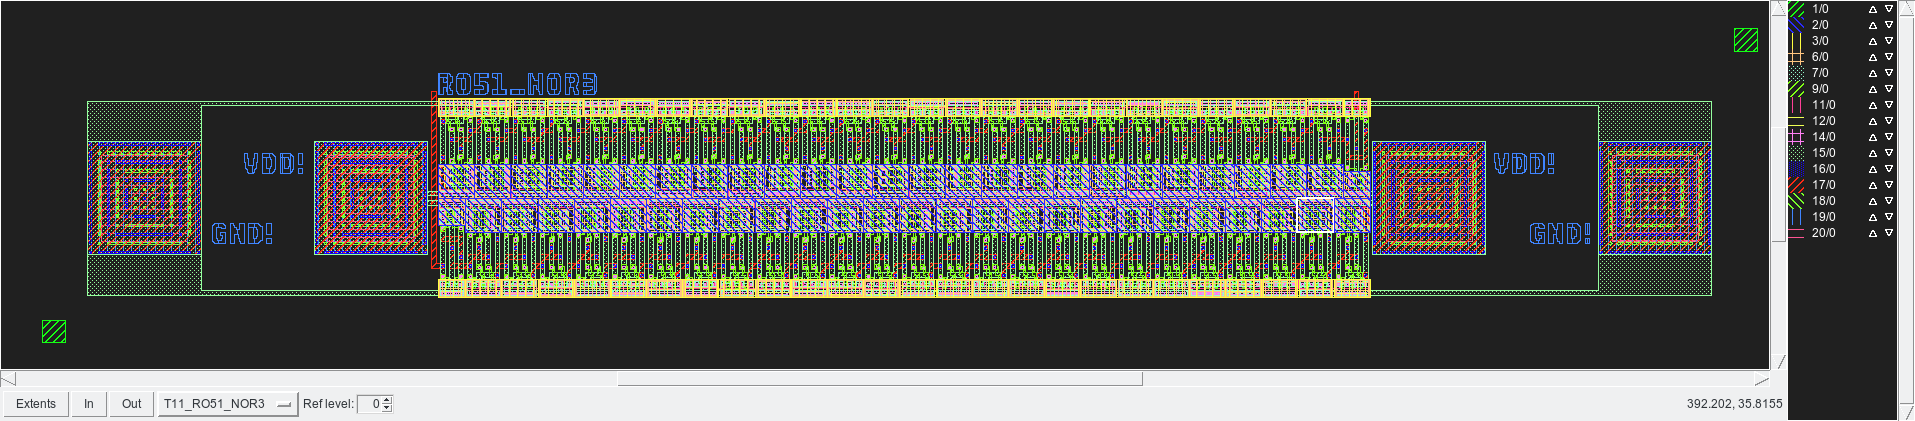
\includegraphics[width=\textwidth]{images/Screenshot_20181219_184458.png}
	\end{center}
\end{frame}

\begin{frame}{Example: NOR3 ring oscillator}
	\begin{center}
		\textbf{Wells (nwell/pwell):}

		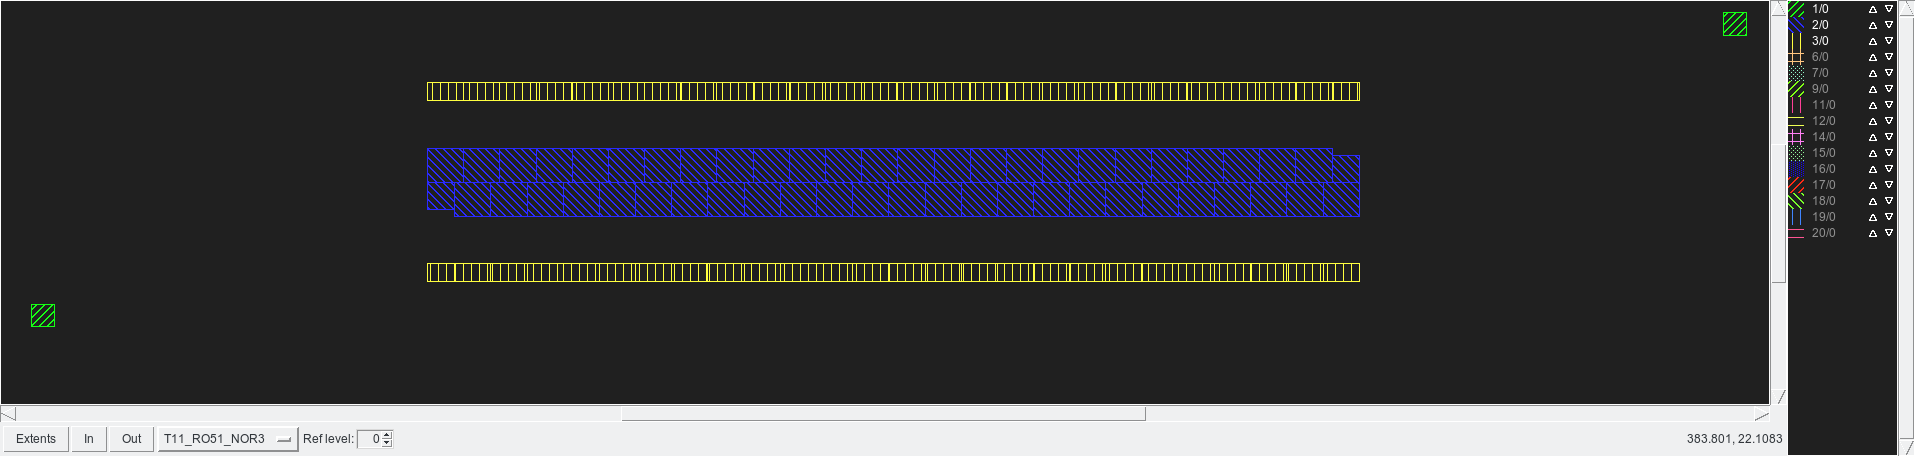
\includegraphics[width=\textwidth]{images/Screenshot_20181221_124540.png}
	\end{center}
\end{frame}

\begin{frame}{Example: NOR3 ring oscillator}
	\begin{center}
		\textbf{Wells (nwell/pwell):}

		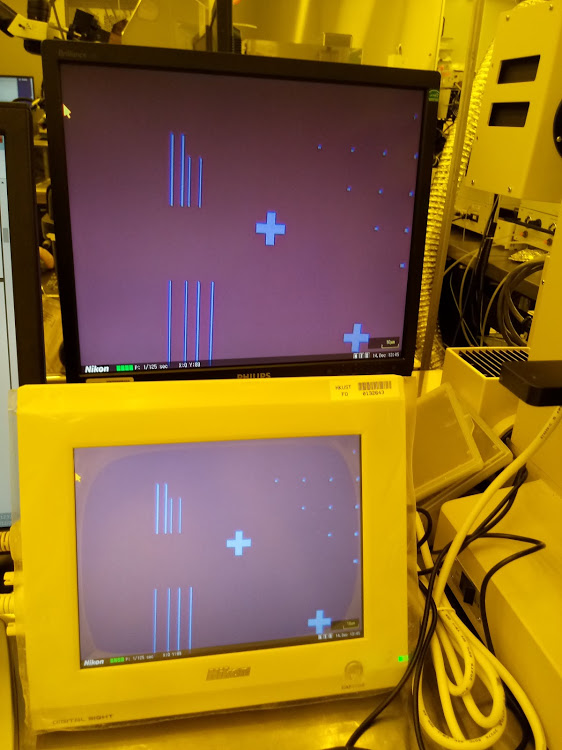
\includegraphics[width=0.25\textwidth]{images/20181214_125705.jpg}
	\end{center}
\end{frame}

\begin{frame}{Example: NOR3 ring oscillator}
	\textbf{Recipe for nwell:}
	\begin{itemize}
		\item Coat with implant resist (soft bake 60 seconds, 110\textdegree{}C)
		\item Expose nwell-mask
		\item Puddle develop 69 seconds and hard bake 60 seconds at 120\textdegree{}C
		\item Implant Phosphorus, $2.33 \times 10^{12} cm^{-2}$ @ 70keV
		\item Strip resist with plasma asher or 20 minutes in 120\textdegree{}C hot sulfuric acid
	\end{itemize}
	\textbf{Note:} Alternatively predisposition can be used
\end{frame}

\begin{frame}{Example: NOR3 ring oscillator}
	\textbf{Recipe for pwell:}
	\begin{itemize}
		\item Coat with implant resist (soft bake 60 seconds, 110\textdegree{}C)
		\item Expose pwell-mask
		\item Puddle develop 69 seconds and hard bake 60 seconds at 120\textdegree{}C
		\item Implant Boron, $1.93 \times 10^{12} cm^{-2}$ @ 40keV
		\item Strip resist with plasma asher or 20 minutes in 120\textdegree{}C hot sulfuric acid
		\item Diffuse both wells together for 4 hours at 1050\textdegree{}C in inert atmosphere ($N_2$) 
	\end{itemize}
	\textbf{Note:} Alternatively predisposition can be used
\end{frame}

\begin{frame}{The Fick's equation}
\begin{center}
	\begingroup
	\huge
	$\frac{\partial N}{\partial t} = D \cdot \frac{\partial^2 N}{\partial x^2}$
	\endgroup
\end{center}
\end{frame}

\definecolor{LightCyan}{rgb}{0.88,1,1}

\begin{frame}{The Fick's equation}
\begin{center}
	$x_l(t) = 2 \cdot \sqrt{D_e \cdot t} = 2 \cdot \sqrt{D_0 \cdot \exp\left(-\frac{E_a}{k \cdot T}\right) \cdot t}$ \\
	\begin{tabular}{|c|c|c|}
		\hline
		\textbf{Element} &
		$D_0$ $\left[\frac{cm^2}{s}\right]$ &
		$E_a$ $\left[eV\right]$ \\
		\hline
		\rowcolor{LightCyan}
		P &
		10.50 &
		3.69 \\
		\hline
		As &
		0.32 &
		3.56 \\
		\hline
		Sb &
		5.60 &
		3.95 \\
		\hline
		\rowcolor{LightCyan}
		B &
		10.50 &
		3.69 \\
		\hline
		Al &
		8.00 &
		3.47 \\
		\hline
		Ga &
		3.60 &
		3.51 \\
		\hline
		Cu &
		0.0025 &
		0.65 \\
		\hline
	\end{tabular}
\end{center}
\end{frame}

\begin{frame}{The Fick's equation}
	\begin{center}
		\begingroup
		\huge
		$N(x,t)=\frac{Q}{\sqrt{\pi \cdot D_e \cdot t}} \cdot \exp\left(\frac{-x^2}{4 \cdot D_e \cdot t}\right)$
		\endgroup
	\end{center}
\end{frame}

\begin{frame}{The Fick's equation}
	\begin{center}
		For the concentration within the channel may $x=0$

		This results in the concentration at the surface (around 100nm deep $\ll$ 2 microns)

		$ N = \frac{Q}{\sqrt{\pi \cdot D_e \cdot t}} $

		Or the implant dosage:

		$ Q = N \cdot \sqrt{\pi \cdot D_e \cdot t} $
	\end{center}
\end{frame}

\begin{frame}{The Fick's equation}
	\begin{center}
		Fixed source diffusion:

		$ x_j = 2 \cdot\sqrt{D \cdot t \cdot \ln\left(\frac{N_0}{N_B}\right)} $

		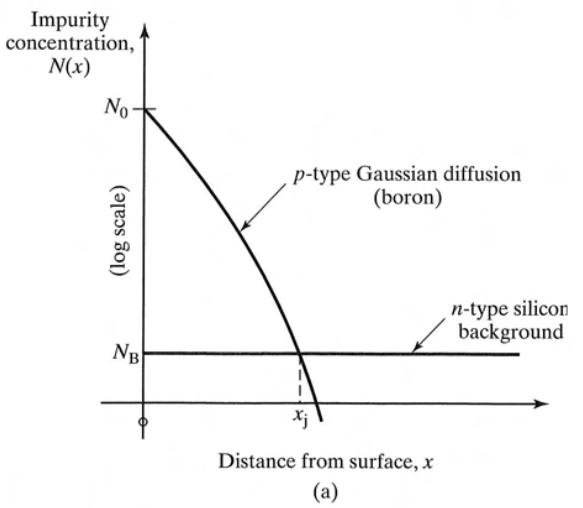
\includegraphics[width=0.25\textwidth]{images/well_formation1.png}
		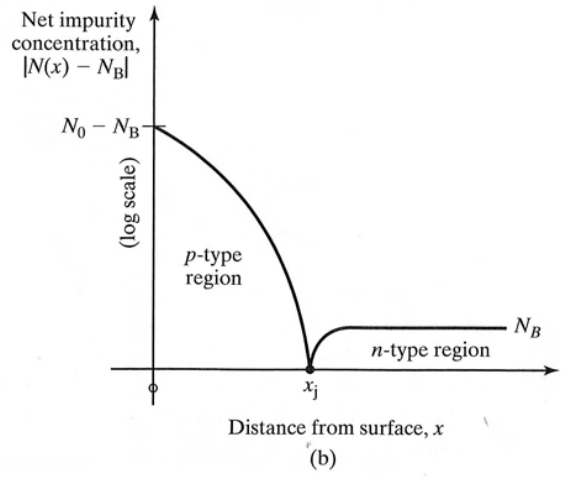
\includegraphics[width=0.25\textwidth]{images/well_formation2.png}
	\end{center}
\end{frame}

\begin{frame}{Threshold calculation}
	\begin{center}
		\textbf{PMOS}

		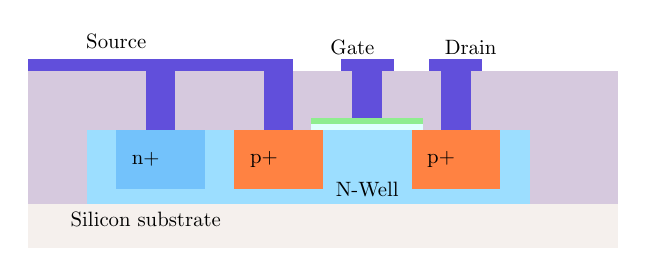
\begin{tikzpicture}[node distance = 3cm, auto, thick, scale=0.75, every node/.style={transform shape}]
			% substrate
\fill[substrate] (0,0) rectangle (10,2);
\node at (2,0.5) {Silicon substrate};

% n-well
\fill[nwell] (1,0.75) rectangle (8.5,2);
\node at (5.75,1) {N-Well};

% body
\fill[nimplant] (1.5,1) rectangle (3,2);
\node at (2,1.5) {n+};
% source
\fill[pimplant] (3.5,1) rectangle (5,2);
\node at (4,1.5) {p+};
% drain
\fill[pimplant] (6.5,1) rectangle (8,2);
\node at (7,1.5) {p+};
%% gate:
% gate oxide
\fill[gateoxide] (4.8,2) rectangle (6.7,2.1);
% gate poly
\fill[poly] (4.8,2.1) rectangle (6.7,2.2);

% metals ground
\fill[metal1] (2,2) rectangle (2.5,3);
\fill[metal1] (4,2) rectangle (4.5,3);
\fill[metal1] (0,3) rectangle (4.5,3.2); % connection pad GND

\fill[metal1] (5.5,2.2) rectangle (6,3);
\fill[metal1] (5.3,3) rectangle (6.2,3.2); % connection pad VG

\fill[metal1] (7,2) rectangle (7.5,3);
\fill[metal1] (6.8,3) rectangle (7.7,3.2); % connection pad VDD

% isolation oxides:
\fill[isolationoxide] (0,2) rectangle (2,3);
\fill[isolationoxide] (2.5,2) rectangle (4,3);
\fill[isolationoxide] (4.5,2) rectangle (4.8,3);
\fill[isolationoxide] (4.8,2.2) rectangle (5.5,3);
\fill[isolationoxide] (6,2.2) rectangle (6.7,3);
\fill[isolationoxide] (6.7,2) rectangle (7,3);
\fill[isolationoxide] (7.5,2) rectangle (10,3);

\node at (1.5,3.5) {Source};
\node at (5.5,3.4) {Gate};
\node at (7.5,3.4) {Drain};

% trench
\fill[isolationoxide] (0,0.75) rectangle (1,2);
\fill[isolationoxide] (8.5,0.75) rectangle (10,2);;
		\end{tikzpicture}
	\end{center}
\end{frame}

\begin{frame}{Threshold calculation}
	\begin{center}
		\textbf{PMOS}

		\begin{equation}
			\left| \phi_F \right| = V_T \ln\frac{N_d}{n_i}
		\end{equation}

		\begin{equation}
			V_T
			=
			V_{FB}
			-
			2 \cdot \left| \phi_F \right|
			-
			\frac{
			\sqrt{2 \cdot \epsilon_s  \cdot q \cdot N_d \cdot \left( 2 \cdot \left| \phi_F \right| - V_{SB}\right) }
			}{C_{ox}}
		\end{equation}

		\begin{equation}
			V_{FB} = -\left( \frac{E_g}{2} - \phi_F \right) - \frac{Q_{SS}}{C_{ox}}
		\end{equation}

	\end{center}
\end{frame}

\begin{frame}{Threshold calculation}
	\begin{center}
		\textbf{NMOS}

		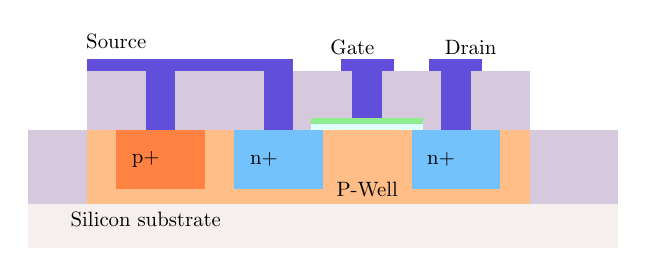
\begin{tikzpicture}[node distance = 3cm, auto, thick, scale=0.75, every node/.style={transform shape}]
			% substrate
\fill[substrate] (0,0) rectangle (10,2);
\node at (2,0.5) {Silicon substrate};
% p-well
\fill[pwell] (1,0.75) rectangle (8.5,2);
\node at (5.75,1) {P-Well};
% body
\fill[pimplant] (1.5,1) rectangle (3,2);
\node at (2,1.5) {p+};
% source
\fill[nimplant] (3.5,1) rectangle (5,2);
\node at (4,1.5) {n+};
% drain
\fill[nimplant] (6.5,1) rectangle (8,2);
\node at (7,1.5) {n+};
%% gate:
% gate oxide
\fill[gateoxide] (4.8,2) rectangle (6.7,2.1);
% gate poly
\fill[poly] (4.8,2.1) rectangle (6.7,2.2);
% metals ground
\fill[metal1] (2,2) rectangle (2.5,3);
\fill[metal1] (4,2) rectangle (4.5,3);
\fill[metal1] (1,3) rectangle (4.5,3.2); % connection pad GND

\fill[metal1] (5.5,2.2) rectangle (6,3);
\fill[metal1] (5.3,3) rectangle (6.2,3.2); % connection pad VG

\fill[metal1] (7,2) rectangle (7.5,3);
\fill[metal1] (6.8,3) rectangle (7.7,3.2); % connection pad VDD

% isolation oxides:
\fill[isolationoxide] (1,2) rectangle (2,3);
\fill[isolationoxide] (2.5,2) rectangle (4,3);
\fill[isolationoxide] (4.5,2) rectangle (4.8,3);
\fill[isolationoxide] (4.8,2.2) rectangle (5.5,3);
\fill[isolationoxide] (6,2.2) rectangle (6.7,3);
\fill[isolationoxide] (6.7,2) rectangle (7,3);
\fill[isolationoxide] (7.5,2) rectangle (8.5,3);

%field oxides:
% trench
\fill[isolationoxide] (0,0.75) rectangle (1,2);
\fill[isolationoxide] (8.5,0.75) rectangle (10,2);

\node at (1.5,3.5) {Source};
\node at (5.5,3.4) {Gate};
\node at (7.5,3.4) {Drain};
		\end{tikzpicture}
	\end{center}
\end{frame}

\begin{frame}{Threshold calculation}
	\begin{center}
		\textbf{NMOS}

		\begin{equation}
			\phi_F = V_T \ln\frac{N_a}{n_i}
		\end{equation}

		\begin{equation}
			V_T
			=
			V_{FB}
			+
			2 \cdot \phi_F
			+
			\frac{\sqrt{2 \cdot \epsilon_s  \cdot q \cdot N_a \cdot \left( 2 \cdot \phi_F + V_{SB} \right) }}{C_{ox}}
		\end{equation}

		\begin{equation}
			V_{FB} = -\left( \frac{E_g}{2} + \phi_F \right) - \frac{Q_{SS}}{C_{ox}}
		\end{equation}

	\end{center}
\end{frame}

\begin{frame}{SONOS flash}
	\begin{center}
		\textbf{Stands for} \\
		\textbf{S}ilicon \\
		\textbf{O}xide \\
		\textbf{N}itride \\
		\textbf{O}xide \\
		\textbf{S}ilicon \\
    \end{center}
\end{frame}

\begin{frame}{SONOS flash}
	\begin{center}
        \textbf{SONOS NMOS}

        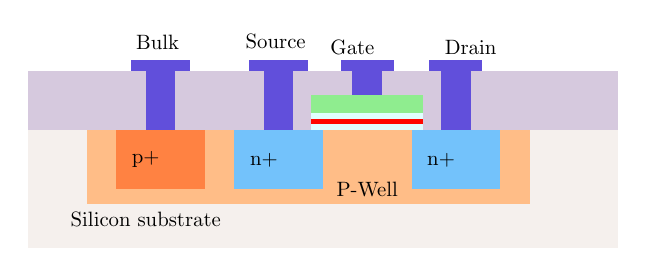
\begin{tikzpicture}[node distance = 3cm, auto, thick, scale=0.75, every node/.style={transform shape}]
			\fill[isolationoxide] (0,0.75) rectangle (10,3);

% substrate
\fill[substrate] (0,0) rectangle (10,2);
\node at (2,0.5) {Silicon substrate};
% p-well
\fill[pwell] (1,0.75) rectangle (8.5,2);
\node at (5.75,1) {P-Well};
% body
\fill[pimplant] (1.5,1) rectangle (3,2);
\node at (2,1.5) {p+};
% source
\fill[nimplant] (3.5,1) rectangle (5,2);
\node at (4,1.5) {n+};
% drain
\fill[nimplant] (6.5,1) rectangle (8,2);
\node at (7,1.5) {n+};
%% gate:

\fill[metal1] (5.5,2.2) rectangle (6,3);
\fill[metal1] (5.3,3) rectangle (6.2,3.2); % connection pad VG

% gate oxide
\fill[gateoxide] (4.8,2) rectangle (6.7,2.1);
\fill[nitride] (4.8,2.1) rectangle (6.7,2.2);
\fill[gateoxide] (4.8,2.2) rectangle (6.7,2.3);
\fill[poly] (4.8,2.3) rectangle (6.7,2.6);

% metal source
\fill[metal1] (4,2) rectangle (4.5,3);
\fill[metal1] (3.75,3) rectangle (4.75,3.2);

\fill[metal1] (2,2) rectangle (2.5,3);
\fill[metal1] (1.75,3) rectangle (2.75,3.2);

\fill[metal1] (7,2) rectangle (7.5,3);
\fill[metal1] (6.8,3) rectangle (7.7,3.2); % connection pad VDD

\node at (2.2,3.5) {Bulk};
\node at (4.2,3.5) {Source};
\node at (5.5,3.4) {Gate};
\node at (7.5,3.4) {Drain};

		\end{tikzpicture}
	\end{center}
\end{frame}

\begin{frame}{SONOS flash}
	\textbf{SONOS NMOS}

	\begin{itemize}
		\item Programming/Erasing happens by changing $Q_{SS}$
		\item A variation of $Q_{SS}$ shifts the threshold voltage
		\item $Q_{SS}$ can be changed by applying an enough high voltage between bulk and gate (approx. 20 V)
		\item High enough voltage tunnels electrons into the nitride
		\item Shifting the threshold voltage away from 0.8 V / -0.8 V makes it stay turned off when a "1" is applied
	\end{itemize}
\end{frame}

\begin{frame}{Example: NOR3 ring oscillator}
	\begin{center}
		\textbf{Isolation (STI):}

		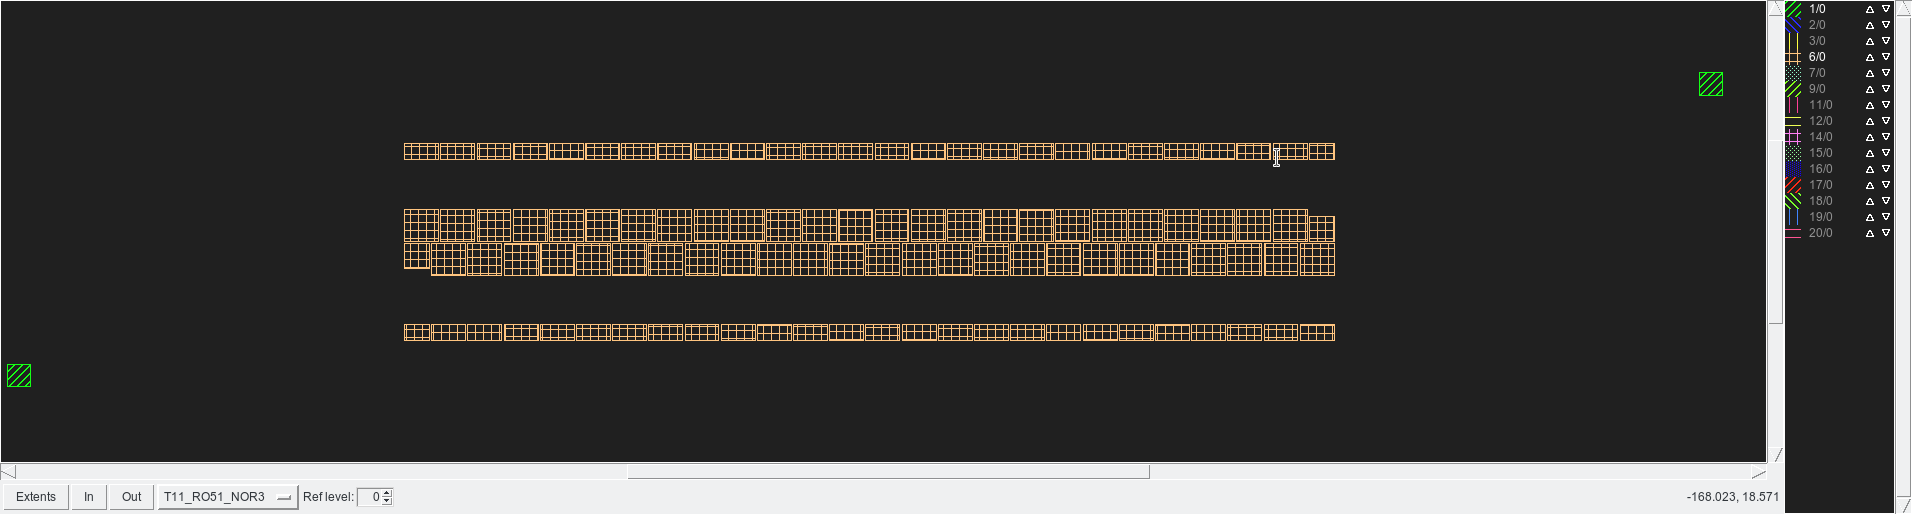
\includegraphics[width=\textwidth]{images/Screenshot_20181220_164222.png}
	\end{center}
\end{frame}

\begin{frame}{Example: NOR3 ring oscillator}
\begin{center}
	\textbf{Isolation (STI):}

	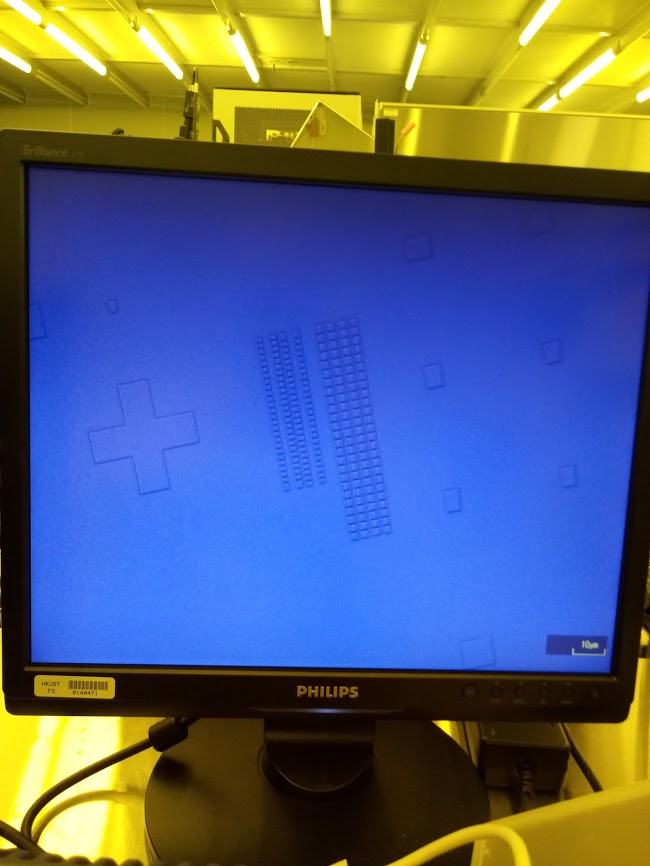
\includegraphics[width=0.25\textwidth]{images/20181219_125354_Burst01.jpg}
	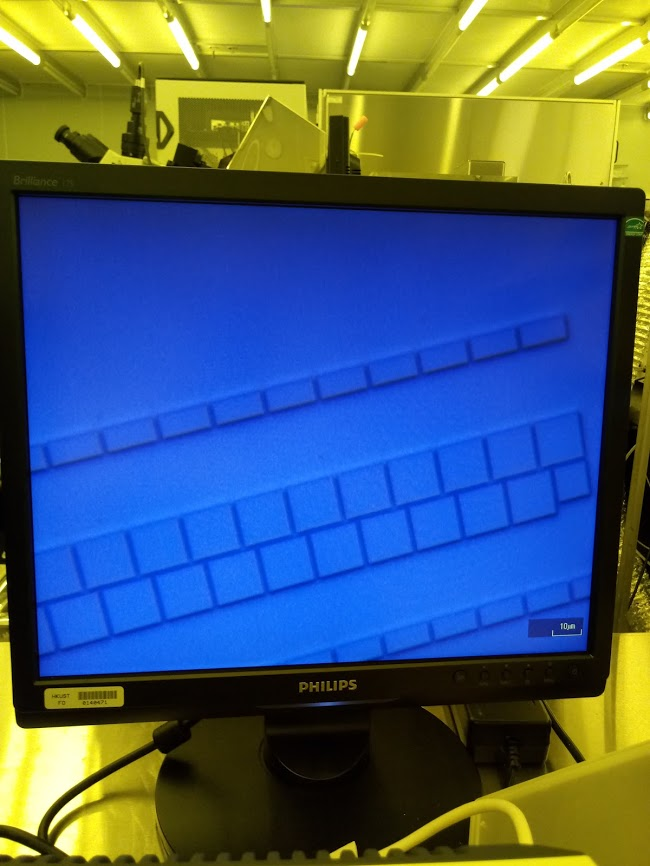
\includegraphics[width=0.25\textwidth]{images/20181219_125758.jpg}
\end{center}
\end{frame}

\begin{frame}{Example: NOR3 ring oscillator}
	\textbf{Recipe for STI:}
	\begin{itemize}
		\item\textbf{Dry}
		\begin{itemize}
			\item Plasma etching recipes are machine specific
			\item Variate the cycles for your recipe to match 2 microns
		\end{itemize}
		\item\textbf{Wet}
		\begin{itemize}
			\item Take TMAH: $ N ( CH _3 ) _4 ^{+} OH ^{−}$ (Tetramethylammonium hydroxide)
			\item Dilute with deionized water with DI:TMAH (3:1)
			\item Heat TMAH (25\%) to 80\textdegree{}C
			\item Dip wafer into the solution for around 6 minutes and 15 seconds (320nm/min, 2 microns)
		\end{itemize}
	\end{itemize}
\end{frame}

\begin{frame}{Example: NOR3 ring oscillator}
\begin{center}
	\textbf{Metal interconnect (metal1):}

	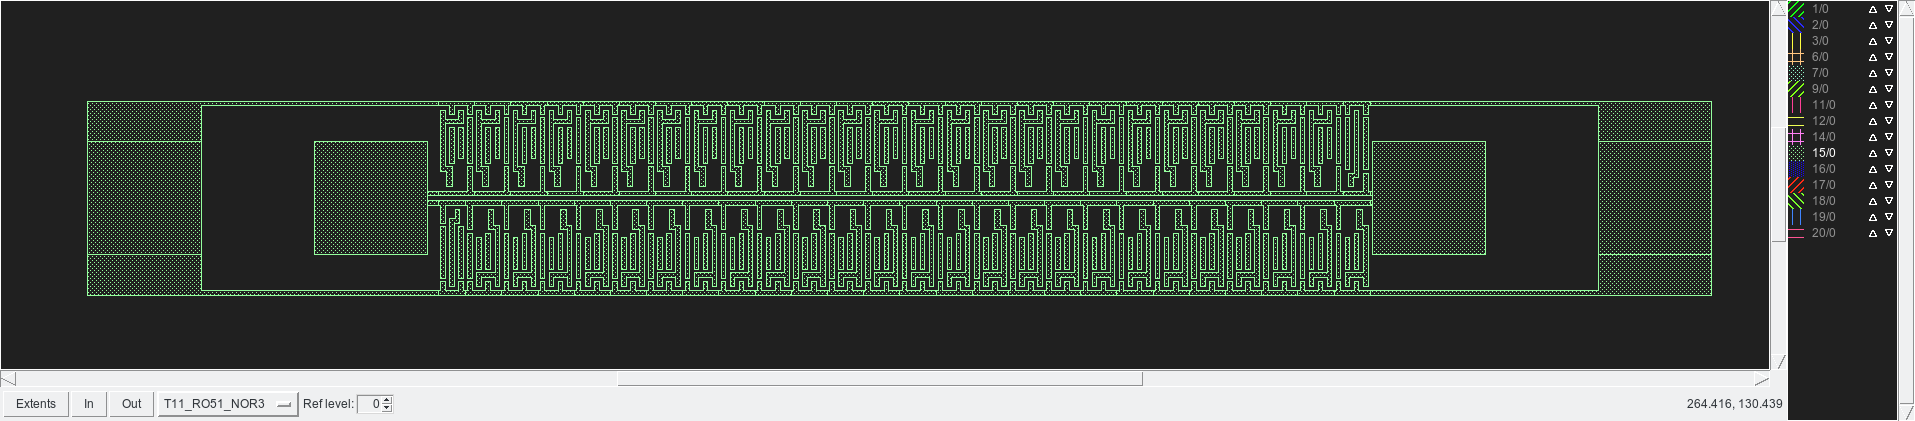
\includegraphics[width=\textwidth]{images/Screenshot_20181219_184526.png}
\end{center}
\end{frame}

\begin{frame}{Example: NOR3 ring oscillator}
\begin{center}
	\textbf{Metal interconnect (metal1):}

	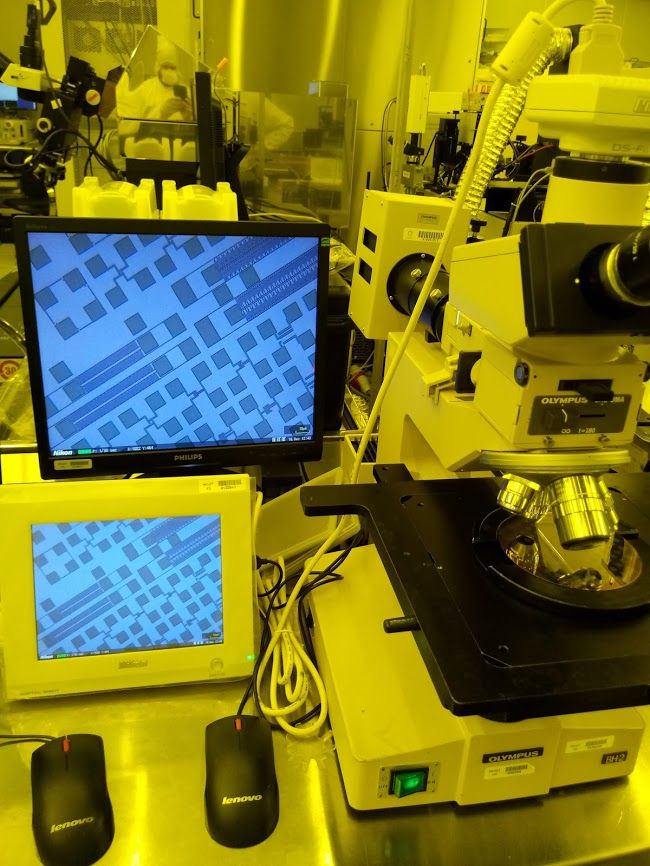
\includegraphics[width=0.25\textwidth]{images/20181218_115931.jpg}
	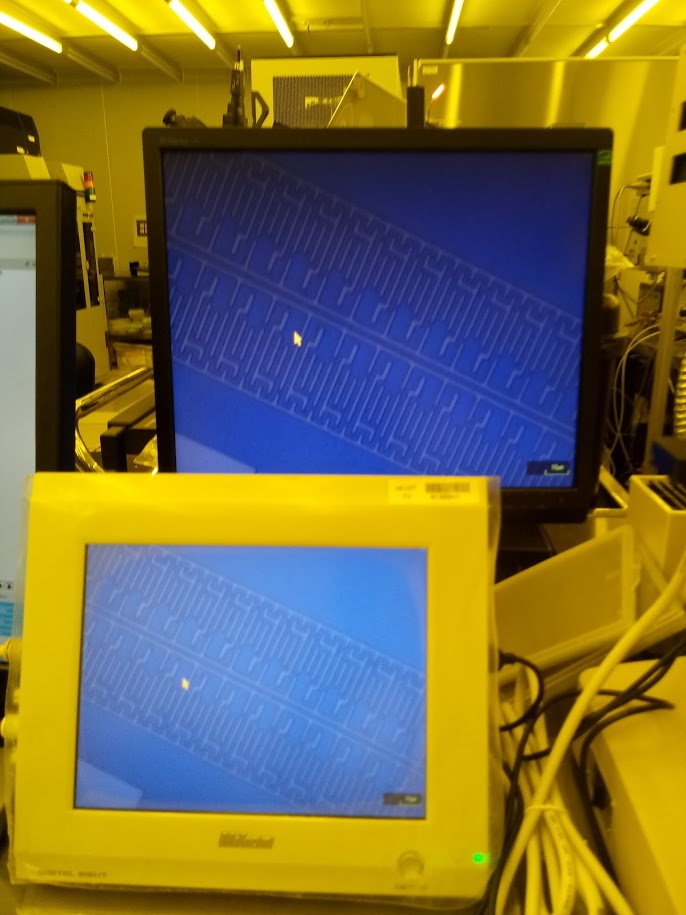
\includegraphics[width=0.25\textwidth]{images/20181218_161016.jpg}
\end{center}
\end{frame}

\begin{frame}{Example: NOR3 ring oscillator}
	\textbf{Recipe for metal interconnects:}

	\begin{itemize}
		\item Make a vacuum (low pressure)
		\item Deposit 100nm Aluminum
		\item Deposit 30nm Titanium over the Aluminum
		\item Take out of vacuum
		\item Dip into HF:DI (1:10) water solution for a few seconds until Titanium is gone
		\item Dip into FeCl3 or other suitable Aluminum etchant for around 30 seconds until Aluminum is gone
	\end{itemize}
\end{frame}

\begin{frame}{Example: NOR3 ring oscillator}
	\textbf{Passivation/Isolation materials}

	\begin{itemize}
		\item Low temperature oxide (LTO)
		\item Phosphosilicate glass (PSG)
	\end{itemize}
	
	\textbf{Can both be wet or dry etched}
\end{frame}

\begin{frame}{Example: NOR3 ring oscillator}
	\textbf{Passivation/Isolation conceptional}

	\begin{center}
		\begin{tikzpicture}[node distance = 3cm, auto, thick, scale=0.25, every node/.style={transform shape}]
			\fill[isolationoxide] (0.0,2.0) rectangle (55.0,\LowerMetal);

\fill[metal1] (1.75,2.0) rectangle (2.25,\LowerMetal);
\fill[metal1] (4.75,2.0) rectangle (5.25,\LowerMetal);
\fill[metal1] (6.0,2.0) rectangle (6.5,\LowerMetal);
\fill[metal1] (7.25,2.0) rectangle (7.75,\LowerMetal);

\fill[metal1] (10.25,2.0) rectangle (10.75,\LowerMetal);
\fill[metal1] (11.5,2.0) rectangle (12.0,\LowerMetal);
\fill[metal1] (12.75,2.0) rectangle (13.25,\LowerMetal);
\fill[metal1] (15.75,2.0) rectangle (16.25,\LowerMetal);

\fill[metal1] (19.25,2.0) rectangle (19.75,\LowerMetal);
\fill[metal1] (22.1,2.0) rectangle (22.5,\LowerMetal);
\fill[metal1] (23.0,2.0) rectangle (23.5,\LowerMetal);
\fill[metal1] (24.0,2.0) rectangle (24.4,\LowerMetal);

\fill[metal1] (27.1,2.0) rectangle (27.65,\LowerMetal);
\fill[metal1] (28.6,2.0) rectangle (28.9,\LowerMetal);
\fill[metal1] (29.85,2.0) rectangle (30.40,\LowerMetal);
\fill[metal1] (31.35,2.0) rectangle (31.65,\LowerMetal);
\fill[metal1] (32.6,2.0) rectangle (33.4,\LowerMetal);

\fill[metal1] (35.85,2.0) rectangle (36.4,\LowerMetal);
\fill[metal1] (37.35,2.0) rectangle (37.65,\LowerMetal);
\fill[metal1] (38.6,2.0) rectangle (38.9,\LowerMetal);
\fill[metal1] (39.85,2.0) rectangle (40.15,\LowerMetal);
\fill[metal1] (41.15,2.0) rectangle (41.6,\LowerMetal);

\fill[metal1] (43.25,2.0) rectangle (43.75,\LowerMetal);
\fill[metal1] (47.25,2.0) rectangle (47.75,\LowerMetal);

\fill[metal1] (49.0,2.0) rectangle (49.5,\LowerMetal);
\fill[metal1] (53.5,2.0) rectangle (54.0,\LowerMetal);

% wires
\fill[metal1] (1.5,\LowerMetal) rectangle (5.5,\UpperMetal);
\fill[metal1] (5.75,\LowerMetal) rectangle (6.75,\UpperMetal);
\fill[metal1] (7.0,\LowerMetal) rectangle (11.0,\UpperMetal);
\fill[metal1] (11.25,\LowerMetal) rectangle (12.25,\UpperMetal);
\fill[metal1] (12.5,\LowerMetal) rectangle (16.5,\UpperMetal);
\fill[metal1] (19.0,\LowerMetal) rectangle (22.5,\UpperMetal);
\fill[metal1] (22.75,\LowerMetal) rectangle (23.75,\UpperMetal);
\fill[metal1] (24.0,\LowerMetal) rectangle (25.75,\UpperMetal);

\fill[metal1] (26.25,\LowerMetal) rectangle (27.75,\UpperMetal);
\fill[metal1] (28.00,\LowerMetal) rectangle (29.25,\UpperMetal);
\fill[metal1] (29.60,\LowerMetal) rectangle (30.55,\UpperMetal);
\fill[metal1] (30.75,\LowerMetal) rectangle (32.25,\UpperMetal);
\fill[metal1] (32.50,\LowerMetal) rectangle (34.00,\UpperMetal);

\fill[metal1] (35.00,\LowerMetal) rectangle (36.45,\UpperMetal);
\fill[metal1] (36.75,\LowerMetal) rectangle (38.0,\UpperMetal);
\fill[metal1] (38.25,\LowerMetal) rectangle (39.5,\UpperMetal);
\fill[metal1] (39.75,\LowerMetal) rectangle (40.90,\UpperMetal);
\fill[metal1] (41.10,\LowerMetal) rectangle (42.25,\UpperMetal);

\fill[metal1] (43.0,\LowerMetal) rectangle (44.5,\UpperMetal);
\fill[metal1] (46.5,\LowerMetal) rectangle (48.0,\UpperMetal);

\fill[metal1] (48.75,\LowerMetal) rectangle (50.25,\UpperMetal);
\fill[metal1] (52.75,\LowerMetal) rectangle (54.25,\UpperMetal);

\input{tikz_process_steps/nimplant.a.tex}

\node at (5,1.65) {p+};
\shade[upper left = pimplant, upper right = pimplant, lower right = nwell, lower left = nwell,] (4.5,1.8) rectangle (5.75,2);
\shade[upper left = pimplant, upper right = pimplant, lower right = poly, lower left = poly,] (5.75,2.7) rectangle (6.75,3.0);
\shade[upper left = pimplant, upper right = pimplant, lower right = nwell, lower left = nwell,] (6.75,1.8) rectangle (8.0,2);

\shade[upper left = pimplant, upper right = pimplant, lower right = pwell, lower left = pwell,] (15.5,1.8) rectangle (16.5,2);

\shade[upper left = pimplant, upper right = pimplant, lower right = nwell, lower left = nwell,] (22.0,1.8) rectangle (22.6,2);
\shade[upper left = pimplant, upper right = pimplant, lower right = poly, lower left = poly,] (22.75,3.2) rectangle (23.75,3.4);
\shade[upper left = pimplant, upper right = pimplant, lower right = nwell, lower left = nwell,] (23.9,1.8) rectangle (24.5,2);

% npn base
\shade[upper left = pimplant, upper right = pimplant, lower right = pwell, lower left = pwell,] (28.5,1.8) rectangle (29.0,2);
\shade[upper left = pimplant, upper right = pimplant, lower right = pwell, lower left = pwell,] (31.25,1.8) rectangle (31.75,2);

% pnp emitter 1 
\shade[upper left = pimplant, upper right = pimplant, lower right = pwell, lower left = pwell,] (35.75,1.8) rectangle (36.5,2);

% pnp collector
\shade[upper left = pimplant, upper right = pimplant, lower right = pwell, lower left = pwell,] (38.5,1.8) rectangle (39.0,2);

% pnp emitter 2
\shade[upper left = pimplant, upper right = pimplant, lower right = pwell, lower left = pwell,] (41.0,1.8) rectangle (41.75,2);

% diode
\shade[upper left = pimplant, upper right = pimplant, lower right = poly, lower left = poly,] (43.5,3.3) rectangle (45.0,3.5);


\filldraw[line width=0, isolationoxide] (5.75,2.0) -- (5.5,2.0) -- (5.75,3.0);
\filldraw[line width=0, isolationoxide] (6.75,2.0) -- (7.0,2.0) -- (6.75,3.0);

\filldraw[line width=0, isolationoxide] (11.25,2.0) -- (11.0,2.0) -- (11.25,3.0);
\filldraw[line width=0, isolationoxide] (12.5,2.0) -- (12.25,2.0) -- (12.25,3.0);

\filldraw[line width=0, isolationoxide] (22.75,2.4) -- (22.6,2.4) -- (22.75,3.4);
\filldraw[line width=0, isolationoxide] (23.75,2.4) -- (23.9,2.4) -- (23.75,3.4);

\fill[silicide] (1.5,1.9) rectangle (2.5,2);
\fill[silicide] (4.5,1.9) rectangle (5.5,2);
\fill[silicide] (5.75,2.9) rectangle (6.75,3.0);
\fill[silicide] (7,1.9) rectangle (8,2);

\fill[silicide] (10.0,1.9) rectangle (11.0,2);
\fill[silicide] (11.25,2.9) rectangle (12.25,3.0);
\fill[silicide] (12.5,1.9) rectangle (13.5,2);
\fill[silicide] (15.5,1.9) rectangle (16.5,2);

\fill[silicide] (19.0,1.9) rectangle (20.0,2);

\fill[silicide] (22.0,1.9) rectangle (22.6,2.0);
\fill[silicide] (22.75,3.3) rectangle (23.75,3.4);
\fill[silicide] (23.9,1.9) rectangle (24.5,2.0);

\fill[silicide] (27.0,1.9) rectangle (27.75,2.0);
\fill[silicide] (28.5,1.9) rectangle (29.0,2.0);
\fill[silicide] (29.75,1.9) rectangle (30.5,2.0);
\fill[silicide] (31.25,1.9) rectangle (31.75,2.0);
\fill[silicide] (32.5,1.9) rectangle (33.5,2.0);

\fill[silicide] (35.75,1.9) rectangle (36.5,2.0);
\fill[silicide] (37.25,1.9) rectangle (37.75,2.0);
\fill[silicide] (38.5,1.9) rectangle (39.0,2.0);
\fill[silicide] (39.75,1.9) rectangle (40.25,2.0);
\fill[silicide] (41.0,1.9) rectangle (41.75,2.0);

% diode contacts
\fill[silicide] (43.0,3.4) rectangle (44.0,3.5);
\fill[silicide] (47.0,3.4) rectangle (48.0,3.5);

% resistor contacts
\fill[silicide] (49.0,3.4) rectangle (49.5,3.5);
\fill[silicide] (53.5,3.4) rectangle (54.0,3.5);


		\end{tikzpicture}
	\end{center}
\end{frame}

\begin{frame}{Example: NOR3 ring oscillator}
	\textbf{Passivation/Isolation layout}

	\begin{center}
		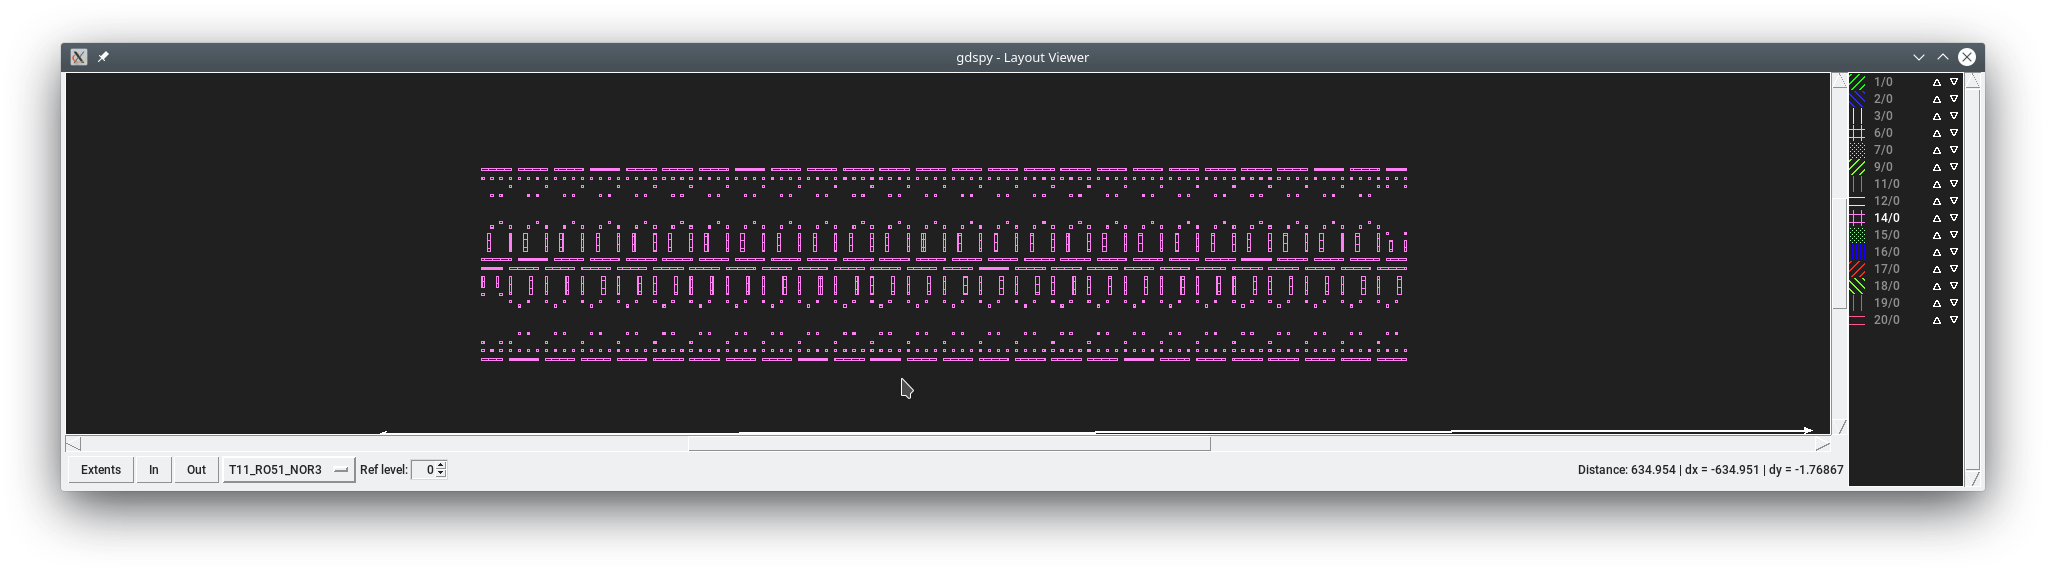
\includegraphics[width=\textwidth]{images/Screenshot_20181225_081522.png}
	\end{center}
\end{frame}

\begin{frame}{Example: NOR3 ring oscillator}
	\textbf{Passivation/Isolation in reality}

	\begin{center}
		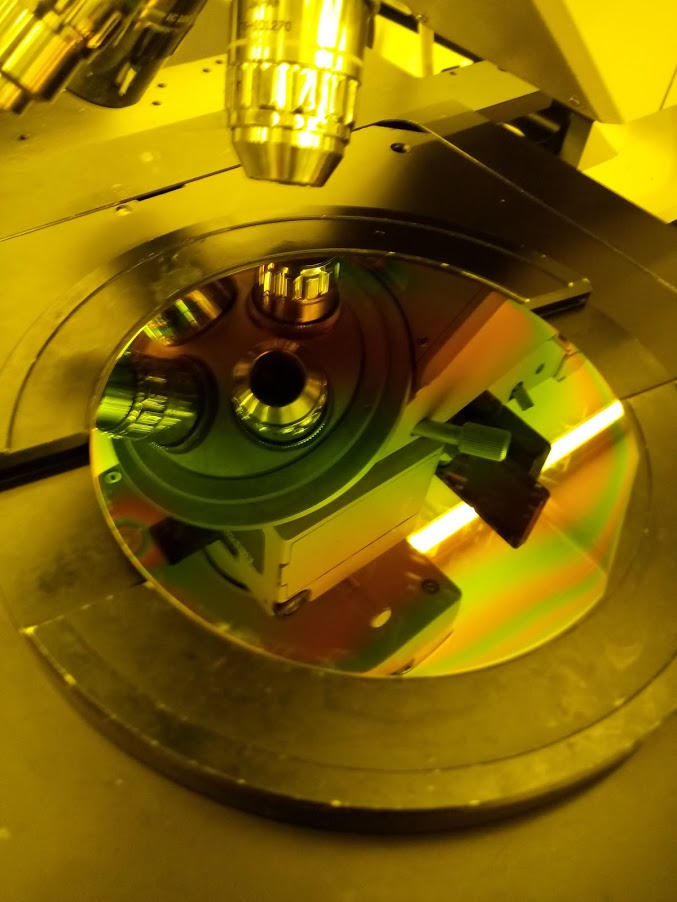
\includegraphics[width=0.25\textwidth]{images/20181220_122500_Burst01.jpg}
	\end{center}
\end{frame}

\begin{frame}{Example: NOR3 ring oscillator}
	\textbf{Passivation/Isolation}

	\begin{center}
		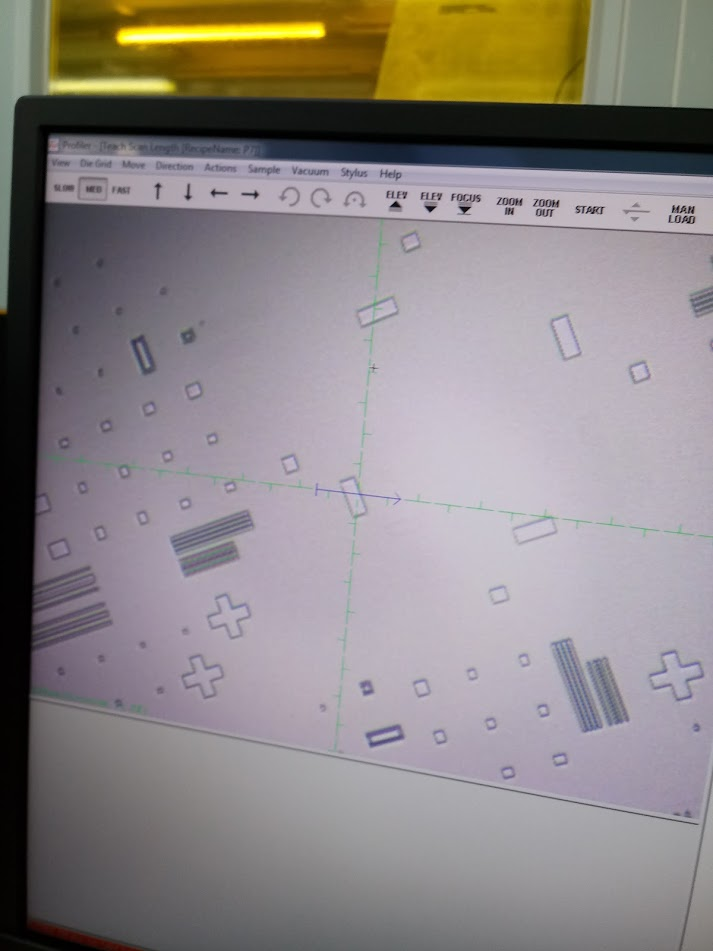
\includegraphics[width=0.25\textwidth]{images/20181220_124056.jpg}
	\end{center}
\end{frame}

\begin{frame}{Example: NOR3 ring oscillator}
	\textbf{Passivation/Isolation}

	\begin{center}
		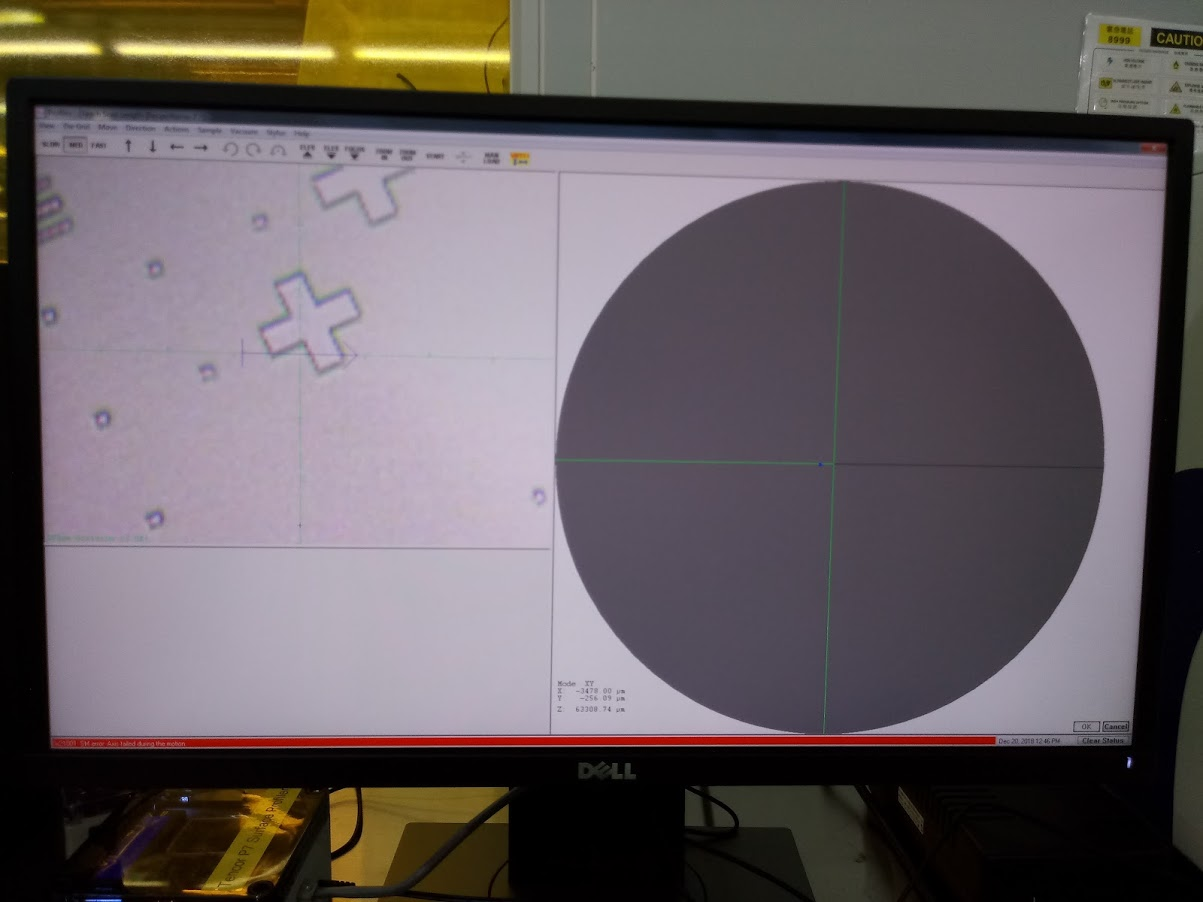
\includegraphics[width=0.4\textwidth]{images/20181220_124600.jpg}
		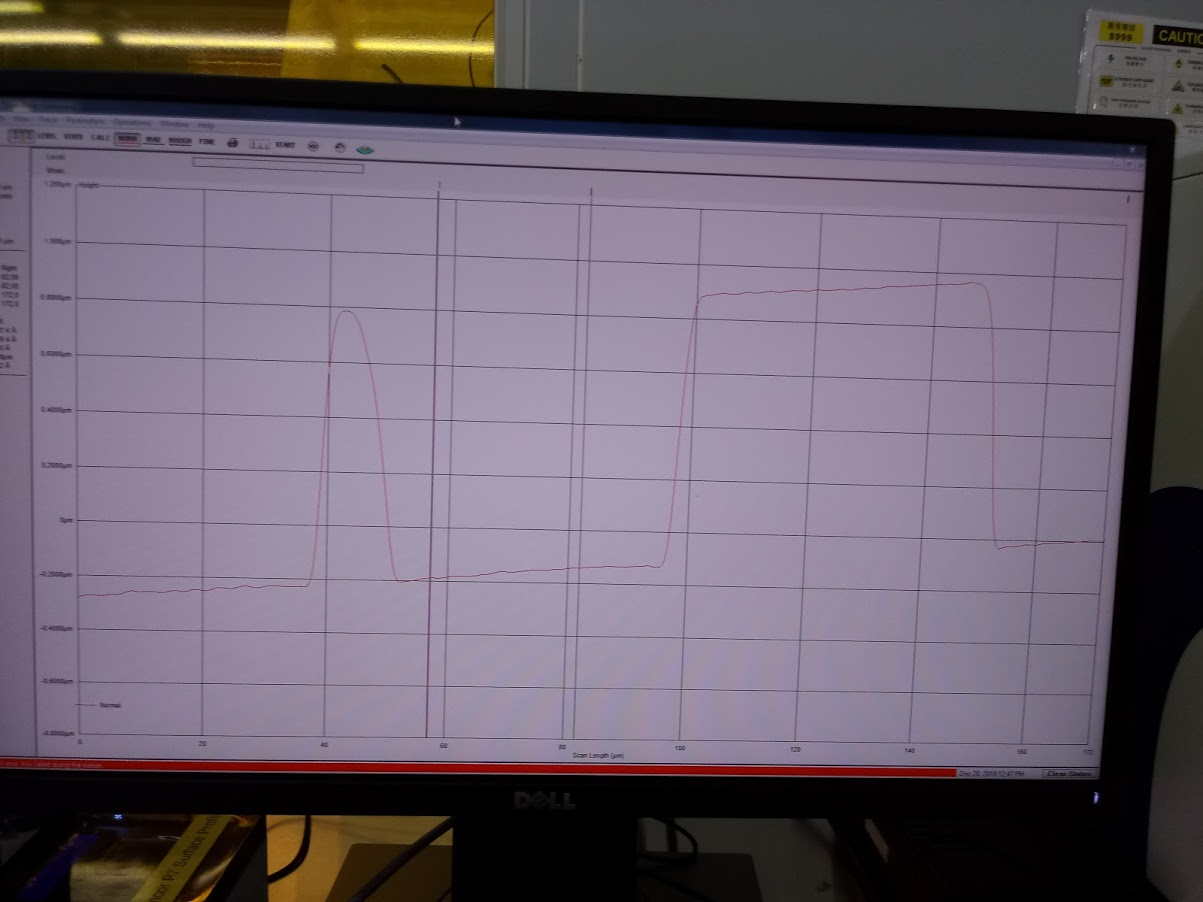
\includegraphics[width=0.4\textwidth]{images/20181220_124638_Burst01.jpg}
	\end{center}
\end{frame}

\begin{frame}{Example: NOR3 ring oscillator}
	\textbf{Passivation/Isolation}

	\begin{itemize}
		\item 1 micron is not enough
		\item 2 more microns need to be deposited
		\item Can be then be etched with BOE after exposure and development
	\end{itemize}
\end{frame}

\begin{frame}{Process}
	\begin{itemize}
        \setlength\itemsep{1em}
		\item https://www.github.com/libresilicon/process ($\rightarrow$ repository)
	\end{itemize}

maintained by leviathanch
\end{frame}


\section[Epilog]{}

\begin{frame}{Next}
	\begin{center}
		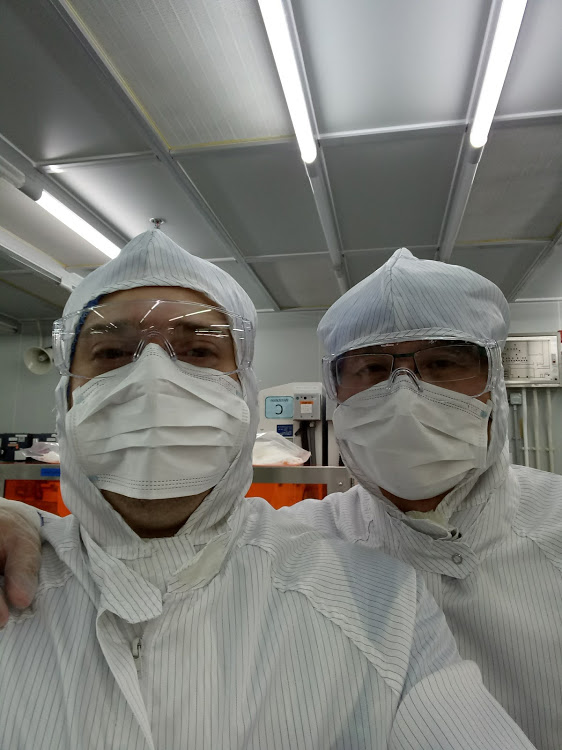
\includegraphics[width=0.25\textwidth]{images/20181210_161139.jpg}

		\textbf{Victor and I}
	\end{center}
\end{frame}

\begin{frame}{Next}
	\cjkfont {
	\large{We will}
	\begin{enumerate}
		\item Finish debugging all the features of PearlRiver \cjkfont(珠江芯片一号)
		\item Create preliminary Verilog and Spice models
		\item Autogenerating standard cells with Popcorn scripts
		\item Building ADCs/DACs and much more analog stuff
		\item Build the North Point MCU \cjkfont(北角芯片)
		\item Build the Sau Mau Ping SoC \cjkfont(秀茂坪芯片)
	\end{enumerate}
	}
\end{frame}

\begin{frame}{Next}
	\begin{center}
		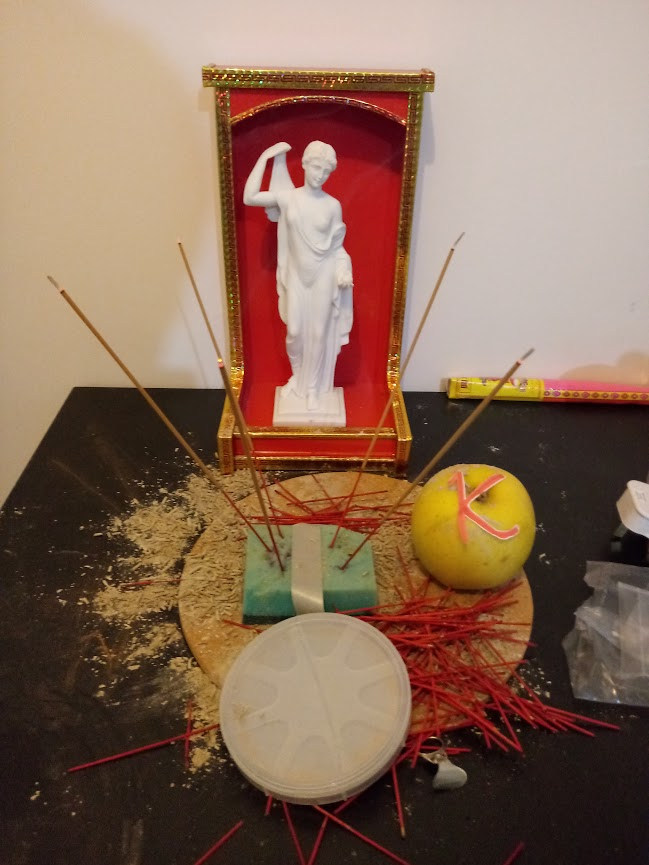
\includegraphics[width=0.3\textwidth]{images/discordia.jpg}

		\textbf{With lots of luck from the goddess}
	\end{center}
\end{frame}

\begin{frame}{North Point \cjkfont(北角芯片)}
	\textbf{Features}

	\begin{itemize}
		\item RISC-V core based on RV32EAC ISA
		\item Pin compatible to ATMega8
		\item Same features as ATMega8
		\item Tolerates up to 40V
	\end{itemize}
\end{frame}

\begin{frame}{North Point \cjkfont(北角芯片)}
	\begin{center}
		\begingroup
		\huge
		\textbf{Survey}

		\url{https://survey.libresilicon.com}
		\endgroup
	\end{center}
\end{frame}

\begin{frame}{Future}
	\begin{itemize}
        \setlength\itemsep{1em}
		\item Equipment we are using is ready for going down to 500 nm ($\rightarrow$ 2 nodes shrinking) :-)
	\end{itemize}
\end{frame}

\begin{frame}{Request for Chips}
Which Free and Open Silicon do you like to see also?
	\begin{itemize}
		\item More Analog Stuff? ($\rightarrow$ NE555?, uA741?)
		\item More Digital Stuff? ($\rightarrow$ CD4000-series? LISP-CPU?)
		\item More Mixed-Signal Stuff? ($\rightarrow$ SoC w/ Analog-Digital / Digital-Analog Converter?)
		\item ?
	\end{itemize}
Keep on track, let us know your wish list!
	\begin{center}
		\textbf{Mailing List:} \url{http://list.o2s.ch/mailman/listinfo/libre-silicon-devel}
	\end{center}
\end{frame}

\begin{frame}{Thanks!}
	\begin{center}
		\textbf{\cjkfont{非常感谢你们!}} \\
		\textbf{Thank you very much!} \\
		\textbf{Vielen herzlichen Dank!} \\
		
\includegraphics[width=100pt]{images/cat.png}
	\end{center}
\end{frame}

\end{document}
